\documentclass[10pt, letterpaper]{article}

% Inhaltsverzeichnis für Pakettypen (nur für Übersicht im Header, wird nicht im Dokument angezeigt)
% 1. Seitenlayout und Ränder
% 2. Sprache und Zeichensatz
% 3. Mathematik und Theorem-Umgebungen
% 4. Eigene Makros
% 5. Diagramme und Grafiken
% 6. Tabellen und Aufzählungen
% 7. Inhaltsverzeichnis
% 8. Abschnittsüberschriften
% 9. Abstrakt-Umgebung
% 10. Todos/Notizen
% 11. Rahmen/Box-Umgebungen
% 12. Python-Integration
% 13. Literaturverwaltung
% 14. Hyperlinks
% 15. Absatzeinstellungen
% 16. Umgebungen
% 17  Graphik
% 18  Extra
% 00. Titel und Autor

\usepackage{slashed}

% --- 1. Seitenlayout und Ränder ---
\usepackage[margin=3cm]{geometry}

% --- 2. Sprache und Zeichensatz ---
\usepackage[english]{babel}
\usepackage[T1]{fontenc}
\usepackage[utf8]{inputenc}

% --- 3. Mathematik und Theorem-Umgebungen ---
\usepackage{amsmath, amssymb, amsthm}
\usepackage{mathrsfs}
\DeclareMathOperator{\WF}{WF}

% --- 4. Eigene Makros ---
\usepackage{xcolor}
\newcommand{\SKP}{\langle\cdot,\cdot\rangle}
\newcommand{\id}{\operatorname{id}}
\newcommand{\sgn}{\operatorname{sgn}}
\newcommand{\Ad}{\operatorname{Ad}}
\newcommand{\ad}{\operatorname{ad}}
\newcommand{\R}{\mathbb{R}}
\newcommand{\N}{\mathbb{N}}
\newcommand{\Q}{\mathbb{Q}}
\newcommand{\Z}{\mathbb{Z}}
\newcommand{\C}{\mathbb{C}}
\newcommand{\QU}{\mathbb{H}}
\newcommand{\Cinf}{C^{\infty}}
\newcommand{\Mod}{\mathrm{Mod}}
\newcommand{\Alg}{\mathrm{Alg}}
\newcommand{\Diff}{\mathrm{Diff}}
\newcommand{\Iso}{\mathrm{Iso}}
\newcommand{\Aut}{\mathrm{Aut}}
\newcommand{\End}{\mathrm{End}}
\newcommand{\Hom}{\mathrm{Hom}}
\newcommand{\Cl}{\mathrm{Cl}}
\newcommand{\entwurf}[1]{\textcolor{red}{#1}}
\newcommand{\GL}{\mathrm{GL}}
\newcommand{\Mat}{\mathrm{Mat}}
\newcommand{\SL}{\mathrm{SL}}
\newcommand{\SO}{\mathrm{SO}}
\newcommand{\SU}{\mathrm{SU}}
\newcommand{\Sp}{\mathrm{Sp}}
\newcommand{\Spin}{\mathrm{Spin}}
\newcommand{\Pin}{\mathrm{Pin}}
\newcommand{\Lor}{\mathrm{Lor}}
\newcommand{\Ogroup}{\mathrm{O}}
\newcommand{\U}{\mathrm{U}}

% --- 5. Diagramme und Grafiken ---
\usepackage{graphicx}
\graphicspath{{../../Library/Images/}}
\usepackage[export]{adjustbox}
\usepackage{tikz}
\usetikzlibrary{decorations.pathreplacing, arrows.meta, positioning}
\usepackage{tikz-cd}

% --- 6. Tabellen und Aufzählungen ---
\usepackage{enumitem}
\setlist[itemize]{left=0.5cm}

\newenvironment{romanenum}[1][]
  {%
    \ifx&#1&
    \else
      \textbf{#1}\quad
    \fi
    \begin{enumerate}[label=\roman*)]
  }
  {%
    \end{enumerate}%
  }

% --- 7. Inhaltsverzeichnis ---
\usepackage{tocloft}
\renewcommand{\cftsecfont}{\footnotesize}
\renewcommand{\cftsubsecfont}{\footnotesize}
\renewcommand{\cftsubsubsecfont}{\footnotesize}
\renewcommand{\cftsecpagefont}{\footnotesize}
\renewcommand{\cftsubsecpagefont}{\footnotesize}
\renewcommand{\cftsubsubsecpagefont}{\footnotesize}
\usepackage{etoc}

% --- 8. Abschnittsüberschriften ---
\usepackage{titlesec}
\titleformat{\section}{\normalfont\large\bfseries}{\thesection}{1em}{}
\titleformat{\subsection}{\normalfont\normalsize\bfseries}{\thesubsection}{0.5em}{}
\titleformat{\subsubsection}{\normalfont\normalsize\bfseries}{\thesubsubsection}{0.5em}{}
\setcounter{secnumdepth}{4}

% --- 9. Abstrakt-Umgebung ---
\usepackage{changepage}
\renewenvironment{abstract}
  {
    \begin{adjustwidth}{1.5cm}{1.5cm}
    \small
    \textsc{Abstract. –}%
  }
  {
    \end{adjustwidth}
  }

% --- 10. Todos/Notizen ---
\usepackage{todonotes}
% Hellblau definieren
\definecolor{hellblau}{rgb}{0.3,0.6,1}
\newenvironment{note}{\par\begingroup\color{hellblau}\itshape}{\par\endgroup}

% --- 11. Rahmen/Box-Umgebungen ---
\usepackage{mdframed}
\usepackage{tcolorbox}
\colorlet{shadecolor}{gray!25}

\newenvironment{customTheorem}
  {\vspace{10pt}%
   \begin{mdframed}[
     backgroundcolor=gray!20,
     linewidth=0pt,
     innertopmargin=10pt,
     innerbottommargin=10pt,
     skipabove=\dimexpr\topsep+\ht\strutbox\relax,
     skipbelow=\topsep,
   ]}
  {\end{mdframed}
   \vspace{10pt}%
  }

% --- 12. Python-Integration ---
% (Deaktiviert in dieser Version, aktiviere bei Bedarf)
% \usepackage{pythontex}
% \usepackage[makestderr]{pythontex}

% --- 13. Literaturverwaltung ---
\usepackage{csquotes}
\usepackage[backend=biber, style=alphabetic]{biblatex}
\addbibresource{bibliography.bib}


% --- 14. Hyperlinks ---
\usepackage{hyperref}
\hypersetup{
  colorlinks   = true,
  urlcolor     = blue,
  linkcolor    = blue,
  citecolor    = blue,
  frenchlinks  = true
}

% --- 15. Absatzeinstellungen ---
\usepackage[parfill]{parskip}
\sloppy

% --- 16. Umgebungen ---
\usepackage{thmtools}

\newcommand{\CustomHeading}[3]{%
  \par\medskip\noindent%
  \textbf{#1 #2} \textnormal{(#3)}.\enskip%
}

\newenvironment{DEF}[2]{\CustomHeading{Definition}{#1}{#2}}{}
\newenvironment{PROP}[2]{\CustomHeading{Proposition}{#1}{#2}}{}
\newenvironment{THEO}[2]{\CustomHeading{Theorem}{#1}{#2}}{}
\newenvironment{LEM}[2]{\CustomHeading{Lemma}{#1}{#2}}{}
\newenvironment{KORO}[2]{\CustomHeading{Corollar}{#1}{#2}}{}
\newenvironment{REM}[2]{\CustomHeading{Remark}{#1}{#2}}{}
\newenvironment{EXA}[2]{\CustomHeading{Example}{#1}{#2}}{}
\newenvironment{STUD}[2]{\CustomHeading{Study}{#1}{#2}}{}
\newenvironment{CONC}[2]{\CustomHeading{Concept}{#1}{#2}}{}
\newenvironment{OTH}[2]{\CustomHeading{Other}{#1}{#2}}{}
\newenvironment{EXE}[2]{\CustomHeading{Exercise}{#1}{#2}}{}
\newenvironment{MOT}[2]{\CustomHeading{Motivation}{#1}{#2}}{}
\newenvironment{PROOF}[2]{\CustomHeading{Proof}{#1}{#2}}{}

% --- Unit Umgebung für Source-Inhalte ---
\usepackage{mdframed}
\newmdenv[
  linewidth=1pt,
  topline=false,
  bottomline=false,
  rightline=false,
  leftmargin=0cm,
  rightmargin=0cm,
  skipabove=10pt,
  skipbelow=10pt,
  innertopmargin=0.5\baselineskip,
  innerbottommargin=0.5\baselineskip,
  backgroundcolor=gray!10,
  linecolor=gray
]{unitbox}

\newenvironment{unit}[1]
  {\begin{unitbox}\textbf{Unit #1}\par\smallskip}
  {\end{unitbox}}

% --- 17. ... ---

% --- 18. Extras ---
\usepackage{stmaryrd}
\usepackage{bbold}  % falls du \mathbb{1} nutzen willst

% --- 00. Titel und Autor ---
\title{Einführung in Riemannsche Spin-Geometrie}
\author{Axel Jaschik}
\date{\today}




\begin{document}



\begin{center}
    \Large{Einführung in Riemannsche Spin-Geometrie}\\[10pt]
\end{center}
\vspace{0.1cm}

\begin{center}
     {Herrn Prof. Dr. Bernig: \textit{Riemannsche Geometrie und Lie Gruppen} (Blockseminar WS25/26)}\\
\end{center}


\begin{center}
    \footnotesize{Axel Tim Jaschik \qquad s0852124@stud.uni-frankfurt.de\qquad Matrik.Nr.: 6641832}
\end{center}

\rule{\textwidth}{0.5pt}
\begin{abstract}
Diese Ausarbeitung gibt eine in sich geschlossene Einführung in die Riemannsche Spin-Geometrie mit besonderem Schwerpunkt auf der geometrischen und analytischen Struktur von Dirac-Operatoren. Ausgehend von Diracs ursprünglicher Konstruktion in der relativistischen Quantenmechanik wird motiviert, weshalb Clifford-Algebren und spinorielle Darstellungen notwendige Bestandteile einer physikalisch relevanter Feldgleichungen sind. Orientiert an Diracs Setting wollen wir ein Model eines euklidischen Dirac Operators entwickeln, von welchem sich charakteristische Eigenschaften eines Dirac Operators in der Riemannschen Geometrie ablesen lassen. Ausgehnd von dieser Charakterisierung wollen wird das allgemeine Setting entwickeln, wobei hier im Gegensatz zu den vorherigen global tivialen geometrischen Settings auf die Feinheiten der Globalen Analysis eingegangen werden muss. 

Nach einer kurzen Einführung in Clifford-Algebren, Pin- und Spin-Gruppen werden die Spin-Strukturen auf orientierten Riemannschen Mannigfaltigkeiten sowie die Spinorbündel als assoziierte Vektorbündel zu Spin-Rahmenbündeln entwickelt. Darauf aufbauend werden Spinorzusammenhänge, die sowohl mit dem Levi-Civita-Zusammenhang als auch mit der Clifford-Multiplikation verträglich sind, und der klassische Dirac-Operator eingeführt. Die zuvor festgehaltenen charakteristischen Eigenschaften eines Dirac Operators werden für diesen Differentialoperator diskutiert.

Abschließend wird die Lichnerowicz-Formel bewiesen, welche das Quadrat des Dirac-Operators mit dem Spinor-Laplace-Operator und der skalaren Krümmung in Beziehung setzt. Als Anwendung werden klassische Verschwindungs- und Obstruktionsresultate für Mannigfaltigkeiten mit positiver skalarer Krümmung skizziert.
\end{abstract}
\rule{\textwidth}{0.5pt}
\vspace{0.1cm}


\tableofcontents


\vspace{0.8cm}


\section{Einleitung}

Diese Ausarbeitung soll eine Einführung in die sogenannte \emph{Riemannsche Spin-Geometrie} geben. Da allein die Etablierung der Grundobjekte der Spin-Geometrie einiges an konzeptueller Arbeit erfordert, wird es notwendig sein, an einigen Stellen Details kurz zu referieren und auf die Literatur zu verweisen, um abschließend noch erste interessante Resultate erreichen zu können. 


Wir starten mit $(M,g,\text{Orie})$ eine orientierte Riemannsche Mannigfaltigkeit. Genauer wollen wir in die Riemannische Spin-Geometrie einführen, indem wir eine natürliche Problemstellung untersuchen.

\begin{MOT}{}{Natürlicher Differentialoperator zwischen Vektorbündeln}
  Gibt es ein Paar 
  $$\left( (E,\pi,M,V), D \right)$$
  von $(E,\pi,M,V)$ einem Vektorbündel mit typischer Faser $V$ einem endlichdimensionalen $\mathbb{K}$-Vektorraum und einen Differentialoperator $D\in \mathscr{D}_1(\Gamma(E),\Gamma(E)))$, sodass folgende Eigenschaften durch das Paar erfüllt werden:
  \begin{enumerate}
    \item $D$ ist \emph{intrinsisch}: Der Operator $D$ hängt nur von den \emph{intrinsischen Daten} der orientierten Riemannschen Mannigfaltigkeit ab, also von der Tangentialstruktur, der Metrik, der Orientierung und von daraus kanonisch ableitbaren Daten.

    \item $D^2$ ist \emph{vom Laplace-Typ}: Der quadrierte Operator
    \[
      D^2\in \mathscr{D}_2(\Gamma(E),\Gamma(E)))
    \]
    besitzt dasselbe Prinzipalsymbol wie ein verallgemeinerter Laplace-Operator, also
    \[
      \sigma_2(D^2,\xi)=-\,g_x(\xi^\sharp,\xi^\sharp)\,\id_{E_x}
      =-\,|\xi|_g^2\,\id_{E_x}
      \qquad
      \text{für alle }x\in M,\ \xi\in T_x^*M.
    \]
    Äquivalent bedeutet dies, dass $D^2$ im höchsten Ordnungsterm durch die Riemannsche Metrik bestimmt ist und lokal die Form
    {\color{blue}\[
      D^2=-\sum_{i,j} g^{ij}\,\partial_i\partial_j+\text{Terme niedrigerer Ordnung}
    \]}
    besitzt.
  \end{enumerate}
  Nachfolgend bezeichnen wir ein solches Paar bzw. das jeweilige Vektorbündel und den Differentialoperator als \emph{natürlich}, wenn jene die Eigenschaften erfüllen.
\end{MOT}

Die Riemannische Spin-Geometrie liefert eine Antwort auf diese Frage und entwickelt eine umfassende Theorie auf geeigneten Paaren von Vektorbündeln und Differentialoperatoren mit weitreichenden Resultaten an der Schnittstelle von Differentialgeometrie und Topologie, aber auch in der Mathematischen Physik (Pseudoriemannsche Spin-Geometrie).


Diese Ausarbeitung widmet sich der Entwicklung des kanonischen Paars von Vektorbündel und Differentialoperator, mit welchem die Riemannische Spin-Geometrie klassischer Weise ansetzt: Das \emph{Spinorbündel} und der \emph{Dirac-Operator}.  

\subsection{Wieso ausgerechnet Clifford-Algebren, Spin-Mannigfaltigkeiten, Spinorbündel und Dirac-Operatoren?}

Wir wollen vor der nachfolgenden aufwendigen Konstruktion dieses Paars einen etwas ausführlicheren heuristischen Rahmen zur Orientierung anbieten.


\subsubsection{Laplace-Typ-Bedingung erzwingt Realisierung von Clifford-Relation durch Koeffizientenabbildungen in lokaler Darstellung}

Lassen wir zunächst die Frage nach dem geeigneten Vektorbündel außen vor und betrachten genauer die lokale Version der Laplace-Typ Bedingung, so finden wir direkt die charakterisitische Eigenschaft, die Differentialoperatoren der Spin-Geometrie auszeichnet.

Sei $e_1,...,e_n$ ein ON-Rahmen von $M$. Angenommen wir haben einen natürlichen Differentialoperator $D$, welcher lokal sich darstellen lässt durch
$$D=\sum_{i=1}^n a_i\nabla_{e_i}^E,$$
wobei $a_i$ zunächst lokale Koeffizientenabbildungen sind. Quadrieren liefert:
$$D^2=\left(\sum_{i=1}^n a_i\nabla_{e_i}^E\right)\left(\sum_{j=1}^n a_j\nabla^E_{e_j}\right)=\sum_{i,j=1}^n a_ia_j\nabla^E_{e_i}\nabla^E_{e_j} + \text{Terme niedrigerer Ordnung}$$
Geeignetes Aufspalten der Summen liefert in 2. Ordnung
$$\sum_{i=1}^n a_i^2\nabla^E_{e_i}\nabla^E_{e_i} + \frac{1}{2}\sum_{i\neq j}^n (a_ia_j+ a_ja_i)\nabla^E_{e_i}\nabla^E_{e_j}.$$
Damit der zweite Ordnungsterm die Form eines Laplace-Typ-Operators hat, müssen die gemischten Terme verschwinden und die Diagonalterme die richtige Normierung besitzen. Es werden also charakteristische Antikommutator-Bedingungen erzwungen für die Koeffizientenabbildungen
$$a_i^2=-1 \qquad a_ia_j+a_ja_i = 0\qquad i,j=1,...,n,$$
was zusammengefasst genau eine Realisierung der \emph{Clifford-Relation} ergibt:
$$a_ia_j+a_ja_i=-2\delta_{ij}\id$$
Das hat gravierende Konsequenzen, denn damit zeigt sich die notwendig nicht-triviale Natur der Koeffizientenabbildungen von natürlichen Differentialoperatoren.  

Da es sich insbesondere bei den Koeffizientenabbildungen nicht mehr um skalare Funktionen handeln kann, die punktweise einfach skalar auf $\nabla^E_{X}$ wirken, müssen wir hier eine komplexere Form von Wirkung vermuten, d.h.
$$\left(\left(a_i \nabla^E_{e_i}\right)(s)\right)(x)=a_i(x)\left(\left(\nabla^E_{e_i} s\right)(x)\right)$$
mit 
$$\nabla^E_X s:=(\nabla^E s)(X)\in\Gamma(E)\quad \text{ und }\quad  a_i \in \Gamma( \operatorname{End}(E)),\ a_i(x) \in \operatorname{End}\left(E_x\right)=\operatorname{Hom}\left(E_x, E_x\right) $$
wobei wir nun die $a_i$ Abbildungen nicht mehr als Koeffizientenabbildungen, sondern punktweise als \emph{Koeffizientenendomorphismen} auffassen sollten, welche auf die kovarianten Ableitung des Schnittes in Richtung $X$ angewandt wird und unter sich eine Clifford-Relation realisieren müssen. Die Koeffizientenendomorphismen verhalten sich also wie eine \emph{Realisierung der formalen Clifford-Erzeuger auf dem Vektorraum $E_x$}.

\subsubsection{Realisierte Clifford-Relation erzwingt glatter Bündelabbildung $c:TM\longrightarrow \End(E)$ mit faserweiser Realisierung der Clifford-Relation}


Die bisherige lokale Beschreibung lässt sich nun invariant formulieren. Die Koeffizientenendomorphismen \(a_i(x)\in \End(E_x)\) sollen nicht als voneinander unabhängige Operatoren verstanden werden, sondern als Werte einer faserweise linearen Abbildung
\[
c_x:T_xM\longrightarrow \End(E_x),
\]
welche in einem lokalen orthonormalen Rahmen \(e_1,\dots,e_n\) durch
\[
c_x(e_i):=a_i(x)
\]
gegeben ist. Für einen allgemeinen Tangentialvektor
\[
v=\sum_{i=1}^n v^i e_i\in T_xM
\]
setzt man entsprechend
\[
c_x(v):=\sum_{i=1}^n v^i a_i(x)\in \End(E_x).
\]
Die zuvor aus der Laplace-Typ-Bedingung gewonnenen Relationen
\[
a_i a_j+a_j a_i=-2\delta_{ij}\id_{E_x}
\]
nehmen damit die invariante Form
\[
c_x(v)c_x(w)+c_x(w)c_x(v)=-2g_x(v,w)\id_{E_x}
\qquad (v,w\in T_xM)
\]
an. Damit wird die Clifford-Relation punktweise in \(\End(E_x)\) realisiert.

Damit greift punktweise die universelle Eigenschaft der Clifford-Algebra: Es existiert genau ein Algebra-Homomorphismus
\[
\widetilde c_x:\Cl(T_xM,g_x)\longrightarrow \End(E_x),
\]
dessen Einschränkung auf \(T_xM\subset \Cl(T_xM,g_x)\) wieder \(c_x\) ist. Dies wird durch das kommutative Diagramm
\[
\begin{tikzcd}
T_xM \arrow[r,"\iota_x"] \arrow[dr,"c_x"'] & \Cl(T_xM,g_x) \arrow[d,"\widetilde c_x"] \\
& \End(E_x)
\end{tikzcd}
\]
ausgedrückt, wobei \(\iota_x\) die kanonische Einbettung bezeichnet und $\Cl(T_xM,g_x)$ die von \(T_xM\) erzeugte assoziative Algebra mit der definierenden Relation
\[
vw+w v=-2g_x(v,w)\cdot 1.
\]
Damit wirkt nicht nur jeder Tangentialvektor \(v\in T_xM\) auf der Faser \(E_x\), sondern allgemeiner jedes Element der Clifford-Algebra \(\Cl(T_xM,g_x)\). Äquivalent kann man sagen: \(E_x\) trägt eine Darstellung der Algebra \(\Cl(T_xM,g_x)\), oder auch, \(E_x\) ist ein Modul über \(\Cl(T_xM,g_x)\). Die drei Formulierungen meinen in diesem Zusammenhang dieselbe Struktur und sind äquivalent zu der Forderung nach einer faserweisen linearen Abbildung
\[
c_x:T_xM\longrightarrow \End(E_x),
\]
welche punktweise die Clifford-Relation realisiert.

Auf diese Weise wird aus der lokalen Rechnung eine intrinsische geometrische Forderung: Gesucht ist ein Vektorbündel \(E\to M\), für welches eine glatte Bündelabbildung
\[
c:TM\longrightarrow \End(E),
\]
bzw. eine bilineare Bündelabbildung
\[
c:TM\otimes E\longrightarrow E,
\]
existiert, die faserweise die Clifford-Relation realisiert bzw. äquivalent ein Vektorbündel, dessen Fasern \(E_x\) punktweise Moduln über den Clifford-Algebren \(\Cl(T_xM,g_x)\) tragen, und zwar so, dass diese Struktur glatt von \(x\) abhängt. 


\subsubsection{Herleitung des Zusammenhangs $\nabla^E$ aus Riemannischen Daten}

Die Analyse des Hauptsymbols des quadrierten Operators zeigt, dass ein natürlicher Differentialoperator erster Ordnung nicht nur ein Vektorbündel \(E\to M\), sondern zusätzlich eine faserweise Clifford-Wirkung
\[
c:TM\longrightarrow \End(E)
\]
voraussetzt. 


\subsubsection{Zusammengefasste Problemstellung und Ansatz}

Damit ist jedoch erst ein Teil der benötigten Struktur bestimmt. Denn ein Operator der Form
\[
D=\sum_{i=1}^n c(e_i)\nablaÊ_{e_i}
\]
benötigt darüber hinaus einen Zusammenhang auf \(E\). Soll \(D\) allein aus
der orientierten riemannschen Struktur gewonnen werden, so darf auch dieser
Zusammenhang nicht beliebig gewählt werden, sondern muss sich möglichst
kanonisch aus dem Levi-Civita-Zusammenhang der Riemannischen Mannigfaltigkeit ableiten. 


Gesucht ist also eine Konstruktion eines Vektorbündels \(E\to M\), welches zugleich

\begin{enumerate}
\item eine natürliche Clifford-Wirkung trägt und
\item mit einem aus dem Levi-Civita-Zusammenhang induzierten Zusammenhang
      ausgestattet ist,
\end{enumerate}

wobei beide Strukturen miteinander verträglich sein sollen.

Für die Konstruktion solcher Bündel und Zusammenhänge ist der Übergang zu
einem geeigneten Prinzipalbündel das natürliche geometrische Verfahren.
Aus einem Prinzipalbündel und einer Darstellung auf einem Modellraum erhält
man ein assoziiertes Vektorbündel; ebenso induziert ein Zusammenhang auf dem
Prinzipalbündel einen Zusammenhang auf jedem assoziierten Bündel. 

\emph{Die Frage reduziert sich daher darauf, welches Struktur-Prinzipalbündel und welcher
Modellfaserraum in der vorliegenden Situation die riemannische Geometrie und
die Clifford-Struktur verträglich kodieren.}


\subsubsection{Irreduzible Clifford-Moduln als Modellraumwahl}

Für die Konstruktion eines assoziierten Vektorbündels genügt es jedoch nicht,
einen beliebigen Modellraum zu wählen. Da das gesuchte Bündel eine
Clifford-Wirkung tragen soll, liegt es nahe, bereits auf dem Modellfaserraum
eine entsprechende algebraische Struktur zu fordern. Genauer suchen wir einen
komplexen Vektorraum \(V\) zusammen mit einer Darstellung der
Standard-Clifford-Algebra
\[
\C l_n:=\Cl(\R^n,g_{\mathrm{euc}})\otimes \C.
\]
Denn jeder orientierte orthonormale Rahmen $u=(u_1,\dots,u_n)$ liefert eine isometrische Isomorphie
\[
u:\bigl(\R^n,g_{\mathrm{euc}}\bigr)\xrightarrow{\;\cong\;}(T_xM,g_x),
\qquad
(a^1,\dots,a^n)\longmapsto \sum_{i=1}^n a^i u_i.
\]
Nach der universellen Eigenschaft der Clifford-Algebra induziert dies
kanonisch einen Algebraisomorphismus
\[
\C l_n \xrightarrow{\;\cong\;} \Cl(T_xM,g_x)^\C.
\]
In einem orthonormalen Rahmen werden die punktweisen Clifford-Algebren also
alle durch dasselbe Modell \(\C l_n\) beschrieben. Dabei wählen wir hier für den Modellraum direkt die für die klassische Spin-Geometrie relevanten \emph{irreduziblen Clifford-Moduln} 
$$\Sigma_n\subset \C l_n.$$ 


\subsubsection{Ansatz bzgl. $\SO(n)$-Rahmenbündel und darstellungstheoretische Probleme}

Für eine orientierte riemannsche Mannigfaltigkeit ist das natürliche erste
Struktur-Prinzipalbündel das \(\SO(n)\)-Rahmenbündel 
$$\pi: P^{\SO}(M)\to M$$
mit Fasern
\[P_x^{\SO}(M):=\left\{h:\R^n\to T_xM\;\middle|\;h \text{ ist orientierungserhaltende Isometrie}\right\}.\]
Durch unsere Wahl des irreduziblen Clifford-Moduln als Modellraum tritt jedoch ein wesentliches Problem auf: Die zugehörige Spinor-Darstellung ist im Allgemeinen keine
Darstellung von \(\SO(n)\), sondern nur von \(\Spin(n)\). Daher lässt sich
\(\Sigma_n\) im Allgemeinen nicht direkt als \(\SO(n)\)-assoziierter
Modellfaserraum an \(P^{\SO}(M)\) ankleben.

Für eine orientierte riemannsche Mannigfaltigkeit ist das erste natürliche
Struktur-Prinzipalbündel das Bündel der positiv orientierten orthonormalen
Rahmen
\[
P^{\SO}(M)\to M,
\]
dessen Faser über \(x\in M\) durch
\[
P_x^{\SO}(M)
:=
\left\{
h:\R^n\to T_xM
\;\middle|\;
h \text{ ist orientierungserhaltende Isometrie}
\right\}
\]
gegeben ist. Über dieses Bündel lassen sich alle aus der orientierten
riemannschen Struktur durch gewöhnliche \(\SO(n)\)-Darstellungen gewonnenen
assoziierten Vektorbündel konstruieren.

Wählt man nun als Modellfaserraum einen irreduziblen
Clifford-Modul \(\Sigma_n\) so erhält man auf \(\Sigma_n\) zunächst eine Algebra-Darstellung der Clifford-Algebra
\[
\mu:\C l_n \to \End(\Sigma_n),
\]
Da die Spin-Gruppe \(\Spin(n)\) als Untergruppe $\C l_n^*$ der invertierbaren Elemente in
\(\C l_n\) liegt, kann man diese Darstellung auf \(\Spin(n)\) einschränken.
Auf diese Weise entsteht eine lineare Darstellung
\[
\sigma_n:=\mu|_{\Spin(n)}:\Spin(n)\to \GL(\Sigma_n),
\]
die sogenannte \emph{Spinor-Darstellung}.

Gerade diese Darstellung ist diejenige, welche für die Konstruktion des
gesuchten assoziierten Vektorbündels verwendet werden muss. Denn der gewählte
Modellraum \(\Sigma_n\) wurde nicht unabhängig von der Clifford-Struktur
festgelegt, sondern gerade deshalb gewählt, weil auf ihm die erforderliche
Clifford-Multiplikation bereits algebraisch realisiert ist. Soll diese
Clifford-Struktur global auf ein assoziiertes Bündel übertragen werden, so muss
die Strukturgruppe auf genau demselben Modellraum \(\Sigma_n\) wirken. Die
relevante Gruppenwirkung ist damit nicht beliebig, sondern durch die
Einschränkung der Clifford-Darstellung an \(\Spin(n)\) kanonisch vorgegeben.

Hier zeigt sich nun das entscheidende Hindernis des direkten
\(\SO(n)\)-Ansatzes: Die so entstehende Spinor-Darstellung
\[
\sigma_n:\Spin(n)\to \GL(\Sigma_n)
\]
faktorisiert nicht über die Überlagerungsabbildung
\[
\lambda:\Spin(n)\to \SO(n).
\]
Denn wäre
\[
\sigma_n=\rho\circ \lambda
\qquad\text{für eine Darstellung}\qquad
\rho:\SO(n)\to \GL(\Sigma_n),
\]
so müsste jedes Element des Kerns von \(\lambda\) trivial auf \(\Sigma_n\)
wirken. Insbesondere wäre dann
\[
\sigma_n(-1)=\id_{\Sigma_n}.
\]
Für den irreduziblen Spinorraum gilt jedoch
\[
\sigma_n(-1)=-\id_{\Sigma_n}.
\]
Also ist \(\Sigma_n\) kein \(\SO(n)\)-Darstellungsraum, sondern ein echter
\(\Spin(n)\)-Darstellungsraum.






\subsubsection{Ansatz bzgl. $\Spin(n)$-Prinzipalbündel: Spinstruktur}

Gerade dies legt den alternativen Ansatz nahe, das \(\SO(n)\)-Rahmenbündel
selbst auf ein \(\Spin(n)\)-Prinzipalbündel anzuheben. Da
\[
\lambda:\Spin(n)\to \SO(n)
\]
eine zweifache Überlagerung ist und \(\Sigma_n\) eine natürliche
\(\Spin(n)\)-Darstellung trägt, stellt sich die Frage, ob es ein
\(\Spin(n)\)-Prinzipalbündel \(P^{\Spin}(M)\to M\) gibt, das das
\(\SO(n)\)-Rahmenbündel in einer mit \(\lambda\) verträglichen Weise überlagert.

Die Frage nach einer geeigneten Hebung führt genau auf den Begriff der Spinstruktur, an die 3 Anforderungen gestellt sind:

\begin{enumerate}
\item Eine Spinstruktur soll das orientierte orthonormale Rahmenbündel
      \(P^{\SO}(M)\) entlang der zweifachen Überlagerung
      \(\lambda:\Spin(n)\to\SO(n)\) zu einem \(\Spin(n)\)-Prinzipalbündel
      \(P^{\Spin}(M)\) heben.

\item Ein komplexer irreduzibler \(\Cl_n\)-Modul \(\Sigma_n\) mit zugehöriger
      Spinor-Darstellung \(\sigma_n\) soll dann ein assoziiertes Bündel
      \[
      \Sigma M=P^{\Spin}(M)\times_{\sigma_n}\Sigma_n
      \]
      erzeugen, auf dem die modellhafte Clifford-Wirkung zu einer globalen
      Clifford-Multiplikation \(TM\otimes\Sigma M\to\Sigma M\) absteigt.

\item Schließlich soll der Levi-Civita-Zusammenhang der riemannschen
      Mannigfaltigkeit auf \(P^{\Spin}(M)\) und damit auf \(\Sigma M\)
      angehoben werden, so dass ein natürlicher Spinorzusammenhang und daraus
      der Dirac-Operator entstehen.
\end{enumerate}





\pagebreak


\section{Spin Geometrie}


\subsection{Clifford-Algebren, Spin Gruppe und Spinorraum}



\subsubsection{Clifford-Algebren}

Da wir später punktweise zu jedem Tangentialraum mit eingeschränkter Riemannscher Metrik $(T_pM,g_p)$ eine entsprechende Clifford Struktur benötigen, führen wir die Clifford Algebra allgemein für $\mathbb{K}$-Vektorräume mit symmetrischen Bilinearformen ein: 

\begin{DEF}{}{Clifford Algebra von $(V,\beta)$}
  Let $\mathbb{K}=\mathbb{R}$ or $\mathbb{C}$ and let $V$ be a finite-dimensional $\mathbb{K}$-vector space equipped with a symmetric bilinear form $\beta$.
  A Clifford algebra $\Cl(V,\beta)$ for ($V, \beta$) is a unital $\mathbb{K}$-algebra together with a linear map $\imath: V \rightarrow \Cl(V,\beta)$ such that the following properties hold:
  \begin{enumerate}
    \item $\imath(v)^2=-\beta(v, v) \cdot 1, \quad$ for all $v \in V$, or equivalent for all $v, w \in V$:
    $$\imath(v) \cdot \imath(w)+\imath(w) \cdot \imath(v)=-2 \beta(v, w) \cdot 1, \quad$$
    \item ($A, \imath$) is universal with respect to i), i.e.: Whenever $A$ is a unital $\mathbb{K}$-algebra with a linear map $\imath^{\prime}: V \rightarrow A$ satisfying i) then there exists a unique algebra homomorphism $\phi: \Cl(V,\beta) \rightarrow A$ such that the diagram
    
    \begin{center}
    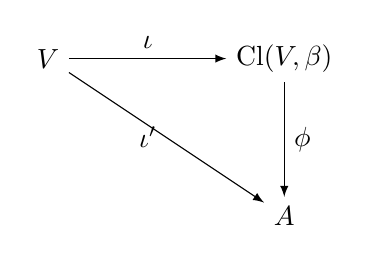
\begin{tikzpicture}[>=latex]

    \node (V) at (0,0) {$V$};
    \node (A) at (3,0) {$\Cl(V,\beta)$};
    \node (Aprime) at (3,-2) {$A$};

    \draw[->] (V) -- node[above] {$\iota$} (A);
    \draw[->] (V) -- node[left] {$\iota'$} (Aprime);
    \draw[->] (A) -- node[right] {$\phi$} (Aprime);

    \end{tikzpicture}
    \end{center}

    commutes. In other words: $A$ is the smallest algebra that satisfies property i).
  \end{enumerate}
  We denote $\Cl_n:=\operatorname{Cl}\left(\mathbb{R}^n, \beta_{\mathrm{eucl}}\right)$ for the Euclidean scalar product.
  
\end{DEF}


\begin{REM}{}{Eigenschaften der Clifford-Algebra}
\begin{enumerate}
  \item \emph{Existenz und Eindeutigkeit der Clifford Algebra}: Diese zeigt man analog zu 
  \item \emph{Basis von $\Cl(V,\beta)$}:
  \item \emph{$\Z^2$-Graduierung der Clifford Algebra und kanonischer Automorphismus}:
\end{enumerate}
\end{REM}






\subsubsection{Pin und Spin Gruppen}

Sei $\mathrm{Cl}_n^{\times}:=\left\{x \in \mathrm{Cl}_n \mid \exists y \in \mathrm{Cl}_n\right.$: $\left.x \cdot y=1\right\}$ die Gruppe der invertierbaren Elemente in der Clifford-Algebra $\mathrm{Cl}_n$. Dann gilt:
\begin{enumerate}
  \item Die Abbildung
  $$
  \begin{aligned}
  \mathrm{Cl}_n \times \mathrm{Cl}_n & \rightarrow \mathrm{Cl}_n \\
  (a, b) & \mapsto a \cdot b
  \end{aligned}
  $$
  ist eine bilineare Abbildung auf endlichdimensionalen $\R$-Vektorräumen und daher glatt.
  \item Die Abbildung
  $$
  \begin{aligned}
  \mathrm{Cl}_n^{\times} & \rightarrow \mathrm{Cl}_n^{\times} \\
  a & \mapsto a^{-1}
  \end{aligned}
  $$
  ist glatt. Damit ist $\mathrm{Cl}_n^{\times}$ eine Lie Gruppe.
  
\end{enumerate}



\begin{REM}{}{Eigenschaften der Spin Gruppe}
  \begin{enumerate}
    \item $\Spin(n)$ ist kompakt, zusammenhängend für $n\geq 2$ und einfach zusammenhängend für $n\geq 3$
    \item $\Spin(n)$ ist eine Lie Untergruppe von $\Cl^*_n$ und $\Pin(n)$
    \item Zweiblättrige Überdeckung von $\SO(n)$
    \item {\color{blue}For $i \neq j$ consider the smooth curve $c: \mathbb{R} \rightarrow \operatorname{Spin}(n)$, defined by

    $$
    t \mapsto\left(\cos (t) e_i+\sin (t) e_j\right) \cdot\left(-e_i\right) .
    $$


    Then $c(0)=e_i \cdot\left(-e_i\right)=1$ and $\dot{c}(0)=e_j \cdot\left(-e_i\right)=e_i \cdot e_j$. We thus have $e_i \cdot e_j \in T_1 \operatorname{Spin}(n) \cong \mathfrak{s p i n}(n)$ for all $i \neq j$.
    The products $\left\{e_i \cdot e_j\right\}, 1 \leq i<j \leq n$ are linearly independent and there are $\frac{1}{2} n(n-1)$ of them. Since $\operatorname{dim}(\mathfrak{s p i n}(n))=\frac{1}{2} n(n-1)$, we conclude that $\left\{e_i \cdot e_j\right\}_{i<j}$ is a basis of $\mathfrak{s p i n}(n)$.}
  \end{enumerate}
\end{REM}


Remark 2.2.4. The subset $\operatorname{Pin}(n) \subset \mathrm{Cl}_n$ is a group with respect to the multiplication in $\mathrm{Cl}_n$. The inverse element to $v_1 \cdot \ldots \cdot v_m$ is given by

$$
\left(v_1 \cdot \ldots \cdot v_m\right)^{-1}=\left(-v_m\right) \cdot \ldots \cdot\left(-v_1\right) \in \operatorname{Pin}(n) .
$$

Remark 2.2.6. By the argument from Remark 2.2.4, $\operatorname{Spin}(n)$ is a subgroup of $\operatorname{Pin}(n)$.


For a fixed $v \in S^{n-1} \subset \mathbb{R}^n$ and any $x \in \mathbb{R}^n$, we have:

$$
v \cdot x \cdot v^{-1}=-v \cdot x \cdot v=-(-x \cdot v-2\langle x, v\rangle 1) \cdot v=-(x-2\langle x, v\rangle v) .
$$


The map $x \mapsto(x-2\langle x, v\rangle v)$ is the reflection about the hyperplane $v^{\perp}$ perpendicular to $v$. In particular, $\left(x \mapsto v \cdot x \cdot v^{-1}\right) \in \mathrm{O}(n)$. For any $a:=v_1 \cdot \ldots \cdot v_m \in \operatorname{Spin}(n)$, the map

$$
x \mapsto a \cdot x \cdot a^{-1}=v_1 \cdot \ldots \cdot v_m \cdot x \cdot v_m^{-1} \cdot \ldots \cdot v_1^{-1}
$$

consists of an even number of hyperplane reflections and is thus contained in $\mathrm{SO}(n)$. We have thus defined a group homomorphism $\varrho: \operatorname{Spin}(n) \rightarrow \operatorname{SO}(n)$ by

$$
\varrho(a) x:=a \cdot x \cdot a^{-1} .
$$

\subsubsection{Spinorraum}


\begin{REM}{}{Einschränkung auf Dimension $n=2m$ gerade}
  Ab hier nehmen wir immer an, dass die orientierte Riemannische Mannigfaltigkeit von Dimension
  $$n=2m\quad \text{gerade}$$ 
  ist und fixieren damit auch die Dimensionen aller anderen relevanten Objekte. {\color{blue} Dies liegt daran, }
\end{REM}

{\color{blue} Nur Case: $\Sigma_n$ für $n$ gerade, $n=2m$}




\begin{DEF}{}{Komplexifizierte Clifford Algebra von $\Cl_n(V,\beta)$}
  Sei $\Cl_n(V,\beta)$ die Clifford-Algebra zu einem reellen Vektorraum $V$ mit symmetrischem Skalarprodukt $\beta$. Die komplexifizierte Clifford-Algebra von $\Cl_n(V,\beta)$ ist definiert durch 
  \[
  \C l(V,g):=\Cl(V,g)\otimes_{\R}\C.
  \]
  Im Falle der Komplexifizierung $\C l_n:= \Cl_n\otimes_{\R}\C$ kann bzgl. der Standardbasis $(e_1,…,e_{2m})$ von $V=\R^n$ aus den Vektoren
  \[
  z_j:=\frac12(e_{2j-1}-i e_{2j}),\qquad
  \bar z_j:=\frac12(e_{2j-1}+i e_{2j})\in \C l_n\qquad  j=1,\dots,m
  \] 
  eine $\C$-Basis von $\C l_n$ konstruiert werden durch die Produkte
  \[
  z(J=(j_1,…,j_k),I=(i_1,…,i_l))=z_{j_1}\cdots z_{j_k}\,\bar z_{i_1}\cdots \bar z_{i_l},
  \qquad k,l=0,\dots,m,
  \]
  mit
  \[
  1\le j_1<\dots<j_k\le m,\qquad 1\le i_1<\dots<i_l\le m,
  \]
\end{DEF}




\begin{DEF}{}{Spinorraum für $n$ gerade}
Sei $\C l_n:=\Cl_n\otimes_{\R}\C$ die komplexifizierte Clifford-Algebra von $\Cl_n$. Wir definieren bzgl. der angegebenen Basis von $\C l_n$ den komplexen Untervektorraum
\[
\Sigma_n:=
\operatorname{span}_{\C}\bigl\{
z(J)=\left(z_{j_1}\cdots z_{j_k}\right)\,\left(\bar z_1\cdots \bar z_m\right)\,\big|\,
k=0,\dots,m,\ 1\le j_1<\dots<j_k\le m
\bigr\}
\subseteq \C l_n.
\]
und nennen diesen den \emph{Spinorraum} in Dimension $n=2m$ und dessen Elemente \emph{Spinoren}.
\end{DEF}

\begin{DEF}{}{Clifford-Modul}
Sei $\C l(V,\beta)$ eine komplexifizierte Clifford-Algebra einer reellen Clifford-Algebra. Ein \emph{(komplexes linkes) Clifford-Modul} über $\C l(V,\beta)$ ist ein komplexer Vektorraum $\Sigma$
zusammen mit einer Algebrenabbildung
\[
\rho:\C l(V,\beta)\longrightarrow \End_{\C}(\Sigma).
\]
Die dadurch induzierte Wirkung
\[
\C l(V,\beta)\times \Sigma\longrightarrow \Sigma,\qquad
(z,\psi)\longmapsto z\cdot \psi:=\rho(z)(\psi)
\]
heißt die \emph{Wirkung der Clifford-Algebra auf $\Sigma$}.

Die \emph{Clifford-Multiplikation} auf einem komplexen Clifford-Modul $\Sigma$ über
$\C l(V,\beta)$ ist die Einschränkung (bzgl. kanonischer Einbettung $V\subset \C l(V,\beta)$)
\[
c:=\rho|_V:V\to \End_{\C}(\Sigma)
\]
und schreibt
\[
c(v)\psi=v\cdot\psi
\qquad (v\in V,\ \psi\in\Sigma).
\]
Durch komplex-lineare Fortsetzung erhält man ebenso
\[
c:V_{\C}\to \End_{\C}(\Sigma).
\]
Die Clifford-Relation lautet dann
\[
c(v)c(w)+c(w)c(v)=-2\,g(v,w)\,\id_{\Sigma}.
\]
Wegen der Clifford-Relation bestimmt $c$ mittels der universellen Eigenschaft von $\C l(V, \beta)$ eindeutig die Darstellung $\rho$.


{\color{blue} Äquivalent gilt für alle $v,w\in V$ und $\psi\in \Sigma$ die Clifford-Relation}
\[
v\cdot (w\cdot \psi)+w\cdot (v\cdot \psi)=-2\,g(v,w)\,\psi.
\]
\end{DEF}


  

\begin{REM}{}{Produktformeln $e_{2 l} \cdot z\left(J\right)$ und $e_{2 l-1} \cdot z\left(J\right)$}
  Für $e_{2l},e_{2l+1}$ aus dem Tupel der Standardbasis von $\R^n$ ist es für spätere Rechnungen hilfreich, Produkte der Form $e_{2 l} \cdot z\left(J\right)$ und $e_{2 l-1} \cdot z\left(J\right)$ zu bestimmen. Dazu unterscheiden wir, ob der Standardbasisvektor in $J$, d.h. in den $z_{j_\nu}=\frac{1}{2}\left(e_{2 j_\nu-1}-i e_{2 j_\nu}\right)$ von $z(J)=\left(z_{j_1}\cdots z_{j_k}\right)\,\left(\bar z_1\cdots \bar z_m\right)$ vorkommt oder nicht:
  \begin{enumerate}
    \item \emph{Case} $e_{(\cdot)}\notin J$: 
    $$
    \begin{aligned}
      e_{2 l} \cdot z\left(J\right) &=i(-1)^\nu z\left(j_1, \ldots, j_\nu, l, j_{\nu+1}, \ldots, j_k\right) \\
      e_{2 l-1} \cdot z\left(J\right) & = (-1)^\nu z\left(j_1, \ldots, j_\nu, l, j_{\nu+1}, \ldots, j_k\right)
    \end{aligned}
    $$
    \item \emph{Case} $e_{(\cdot)}\in J$: 
    $$
    \begin{aligned}
      e_{2 l} \cdot z\left(j_1, \ldots, j_\nu, l, j_{\nu+1}, \ldots, j_k\right)&=(-1)^\nu i z\left(j_1, \ldots, j_\nu, j_{\nu+1}, \ldots, j_k\right)\\
      e_{2 l-1} \cdot z\left(j_1, \ldots, j_\nu, l, j_{\nu+1}, \ldots, j_k\right)&=(-1)^{\nu+1} z\left(j_1, \ldots, j_\nu, j_{\nu+1}, \ldots, j_k\right) .
    \end{aligned}
    $$
  \end{enumerate}
  Diese Formeln lassen sich durch mehrfaches Anwenden der Clifford-Relation beweisen. Durch diese Formeln können wir die Clifford-Multiplikation des Spinorraums $\Sigma_n$ durch Vektoren aus $\R^n$ verstehen.

\end{REM}






\begin{PROP}{}{Der Spinorraum $\Sigma_n$ ist ein Clifford-Modul}
Der Spinorraum $\Sigma_n\subset \C l_n$ ist ein komplexes Clifford-Modul über
$\C l_n$. Genauer gilt:
\begin{enumerate}
    \item $\Sigma_n$ ist ein linkes Ideal in $\C l_n$.
    \item Die Linksmultiplikation in $\C l_n$ induziert eine Darstellung
    \[
    \rho:\C l_n\longrightarrow \End_{\C}(\Sigma_n),
    \qquad
    \rho(z)(\psi):=z\psi .
    \]
    \item Die zugehörige Clifford-Multiplikation ist die Einschränkung
    \[
    c:=\rho|_{\R^n}:\R^n\longrightarrow \End_{\C}(\Sigma_n),
    \qquad
    c(v)(\psi)=v\cdot\psi=v\psi .
    \]
    \item Insbesondere ist $\Sigma_n$ invariant unter der Wirkung von
    $\Spin(n)\subset \Cl_n^0\subset \C l_n$.
\end{enumerate}
\end{PROP}

\begin{proof}
Nach Konstruktion ist $\Sigma_n\subset \C l_n$ unter der Linksmultiplikation mit
Elementen aus $\R^n$ invariant. Da $\C l_n$ als komplexe Algebra von $\R^n$
erzeugt wird, folgt daraus
\[
\C l_n\cdot \Sigma_n\subseteq \Sigma_n.
\]
Also ist $\Sigma_n$ ein linkes Ideal in $\C l_n$.

Damit ist für jedes $z\in \C l_n$ die Linksmultiplikation
\[
\psi\longmapsto z\psi
\]
ein komplex-linearer Endomorphismus von $\Sigma_n$. So erhält man eine wohldefinierte
Algebrenabbildung
\[
\rho:\C l_n\longrightarrow \End_{\C}(\Sigma_n),
\qquad
\rho(z)(\psi):=z\psi.
\]
Folglich ist $\Sigma_n$ ein komplexes Clifford-Modul über $\C l_n$.

Die Clifford-Multiplikation auf $\Sigma_n$ ist per Definition die Einschränkung
dieser Wirkung auf den kanonisch eingebetteten Vektorraum
\[
\R^n\subset \Cl_n\subset \C l_n.
\]
Schreibt man
\[
c:=\rho|_{\R^n},
\]
so gilt für alle $v\in \R^n$ und $\psi\in \Sigma_n$
\[
c(v)(\psi)=v\cdot\psi=v\psi,
\]
wobei rechts das Produkt in der Clifford-Algebra $\C l_n$ steht.

Da schließlich $\Spin(n)\subset \Cl_n^0\subset \C l_n$ gilt, folgt aus der
Invarianz von $\Sigma_n$ unter $\C l_n$ insbesondere die Invarianz unter
$\Spin(n)$.
\end{proof}

\begin{REM}{}{Stärke der Clifford-Wirkung}
Die vorherige Proposition zeigt, dass $\Sigma_n$ durch Linksmultiplikation ein
Clifford-Modul über $\C l_n$ wird, also dass überhaupt eine wohldefinierte
Darstellung
\[
\rho:\C l_n\to \End_{\C}(\Sigma_n)
\]
existiert. Das folgende Resultat ist wesentlich stärker: Es besagt, dass diese
Darstellung bereits die gesamte Endomorphismenalgebra des Spinorraums erfasst,
also ein Isomorphismus
\[
\C l_n \cong \End_{\C}(\Sigma_n)
\]
vorliegt. Damit ist $\Sigma_n$ nicht nur ein Clifford-Modul, sondern das
fundamentale komplexe Clifford-Modul in gerader Dimension.
\end{REM}

\begin{PROP}{}{Clifford-Wirkung auf dem Spinorraum ist vollständig}
Die durch Linksmultiplikation induzierte Abbildung
\[
\rho:\C l_n\longrightarrow \End_{\C}(\Sigma_n),\qquad
\rho(X)(\psi):=X\cdot \psi
\]
ist ein Isomorphismus komplexer Algebren.
\end{PROP}



\begin{DEF}{}{Chiralitätszerlegung des Spinorraums}
Wir definieren für den Spinorraum $\Sigma_n$ die komplexen Untervektorräume
\[
\Sigma_n^{+}
:=
\operatorname{span}_{\C}\{z(j_1,\dots,j_k)\mid k=0,\dots,m,\ k \text{ gerade}\},
\]
und
\[
\Sigma_n^{-}
:=
\operatorname{span}_{\C}\{z(j_1,\dots,j_k)\mid k=0,\dots,m,\ k \text{ ungerade}\}.
\]
Dann heißt
\[
\Sigma_n=\Sigma_n^{+}\oplus \Sigma_n^{-}
\]
die \emph{Chiralitätszerlegung des Spinorraums}. Die Elemente von $\Sigma_n^\pm$
heißen Spinoren \emph{positiver} bzw. \emph{negativer Chiralität}.
\end{DEF}

\begin{PROP}{}{Paritätsverhalten der Clifford-Multiplikation}
Für die Clifford-Multiplikation auf $\Sigma_n$ gilt:
\[
\R^n\cdot \Sigma_n^+ \subset \Sigma_n^-,
\qquad
\R^n\cdot \Sigma_n^- \subset \Sigma_n^+.
\]
Dagegen gilt für den geraden Teil der Clifford-Algebra:
\[
\C l_n^0\cdot \Sigma_n^+ \subset \Sigma_n^+,
\qquad
\C l_n^0\cdot \Sigma_n^- \subset \Sigma_n^-.
\]
\end{PROP}

\begin{DEF}{}{Spinor- und Halbspin-Darstellungen}
Die durch die Einschränkung der Clifford-Wirkung auf $\Spin(n)\subset \Cl_n^0$
induzierte Darstellung
\[
\rho|_{\Spin(n)}:=\sigma_n:\Spin(n)\to \GL(\Sigma_n)
\]
heißt die \emph{Spinor-Darstellung}.

In gerader Dimension induziert die Zerlegung
\[
\Sigma_n=\Sigma_n^+\oplus \Sigma_n^-
\]
die Darstellungen
\[
\sigma_n^\pm:\Spin(n)\to \GL(\Sigma_n^\pm),
\]
die \emph{positive} bzw. \emph{negative Halbspin-Darstellung} heißen.
\end{DEF}



\pagebreak

\subsubsection{Kanoniasches Hermitesches Skalarprodukt auf Spinorraum}



\begin{DEF}{}{Hermitesches Skalarprodukt auf dem Spinorraum}
Wir definieren auf $\Sigma_n$ das \emph{Hermitesche Skalarprodukt}
\[
\langle\cdot,\cdot\rangle_\Sigma:\Sigma_n\times \Sigma_n\to \C
\]
durch die Vorschrift 
$$\langle\phi, \psi\rangle_\Sigma:=\sum_I a_I \overline{b_I}$$
für $\phi=\sum_I a_I z(I), \psi=\sum_I b_I z(I)\in \Sigma_n$ als die eindeutig bestimmte Abbildung, die im ersten Argument komplex-linear, im zweiten Argument komplex-antilinear ist \emph{und} für die die Vektoren
\[
z(j_1,\dots,j_k)
\]
eine \emph{Orthonormalbasis} von $\Sigma_n$ bilden, d.\,h.
\[
\bigl\langle z(j_1,\dots,j_k),\, z(i_1,\dots,i_\ell)\bigr\rangle
=
\delta_{k\ell}\,\delta_{(j_1,\dots,j_k),(i_1,\dots,i_\ell)}.
\]
\end{DEF}

\begin{REM}{}{Eigenschaften des hermiteschen Skalarprodukt auf $\Sigma_n$}
  \begin{enumerate}
    \item \emph{Hermitesche Symmetrie}:
    $$
    \langle\phi, \psi\rangle_\Sigma=\overline{\langle\psi, \phi\rangle} .
    $$
    \item \emph{Positivität}:
    $$
    \langle\phi, \phi\rangle_\Sigma=\sum_I\left|a_I\right|^2 \geq 0,
    $$
    und Gleichheit gilt genau dann, wenn $\phi=0$.
    \item \emph{Clifford-Multiplikation schief-symmetrisch}: Die Clifford-Multiplikation von Spinoren mit Vektoren $X\in\R^n$ ist schief-symmetrisch bzgl $\langle\cdot,\cdot\rangle_\Sigma$:
    $$\langle X \cdot \phi, \psi\rangle_\Sigma= -\langle\phi, X \cdot  \psi\rangle_\Sigma$$
    \item \emph{Orthogonalität der Chiralitätszerlegung}: Da $\Sigma_n^{+}$und $\Sigma_n^{-}$von disjunkten Teilmengen dieser Orthonormalbasis erzeugt werden, ist
    $$
    \Sigma_n=\Sigma_n^{+} \oplus \Sigma_n^{-}
    $$
    eine orthogonale Zerlegung.
    \item \emph{Clifford-Multiplikation ist Isometrie für $X\in S^{n-1}$}: Die Clifford-Multiplikation von Spinoren mit Einheitsvektoren $X\in S^{n-1}$ ist eine Isometrie
    $$\left.\langle X \cdot \phi, X \cdot \psi\rangle_\Sigma=-\langle X \cdot X \cdot \phi, \psi\rangle_\Sigma=-\langle-| X|^2 \phi, \psi\right\rangle=\langle\phi, \psi\rangle_\Sigma$$
    \item \emph{Spinor-Darstellung ist unitär}: Weil $\operatorname{Spin}(n)$ von Produkten von Einheitsvektoren erzeugt wird und diese isometrisch wirken, folgt, dass die Spinor-Darstellung
    $$
    \sigma_n: \operatorname{Spin}(n) \rightarrow \operatorname{GL}\left(\Sigma_n\right)
    $$
    sogar unitär ist relativ zu $\langle\cdot, \cdot\rangle$, d.h. $\sigma_n(\Spin(n))\subset \U(\Sigma_n,\langle\cdot,\cdot\rangle_\Sigma)$ bzw.
    $$\left\langle\sigma_n(g) \phi, \sigma_n(g) \psi\right\rangle_{\Sigma}=\langle\phi, \psi\rangle_{\Sigma} \quad \text{ für alle } \phi, \psi \in \Sigma_n.$$
  \end{enumerate}
  
\end{REM}

\pagebreak



\subsection{Riemannsche Spin-Mannigfaltigkeiten und Spinorbündel}

\subsubsection{Riemannsche Spin-Mannigfaltigkeiten}


Sei $(M,g)$ eine orientierte Riemannsche Mannigfaltigkeit. Für \(x\in M\) setzen wir
\[
P_x^{\SO}(M)
:=
\left\{
h:\R^n\to T_xM
\;\middle|\;
h \text{ ist orientierungserhaltende Isometrie}
\right\}.
\]
Ferner definieren wir
\[
P^{\SO}(M):=\bigsqcup_{x\in M} P_x^{\SO}(M)
\]
und die Projektion
\[
\pi:P^{\SO}(M)\to M,\qquad \pi(h)=x
\quad\text{für }h\in P_x^{\SO}(M).
\]
Auf \(P_x^{\SO}(M)\) wirkt \(\SO(n)\) von rechts durch
\[
P_x^{\SO}(M)\times \SO(n)\to P_x^{\SO}(M),
\qquad
(h,A)\mapsto h\circ A.
\]

\begin{PROP}{}{$\SO(n)$-Rahmenbündel}
Sei $(M,g)$ eine orientierte Riemannsche Mannigfaltigkeit. Für \(x\in M\) setzen wir
\[
P_x^{\SO}(M)
:=
\left\{
h:\R^n\to T_xM
\;\middle|\;
h \text{ ist orientierungserhaltende Isometrie}
\right\}.
\]
Ferner definieren wir
\[
P^{\SO}(M):=\bigsqcup_{x\in M} P_x^{\SO}(M)
\]
und die Projektion
\[
\pi:P^{\SO}(M)\to M,\qquad \pi(h)=x
\quad\text{für }h\in P_x^{\SO}(M).
\]
Auf \(P_x^{\SO}(M)\) wirkt \(\SO(n)\) von rechts durch
\[
P_x^{\SO}(M)\times \SO(n)\to P_x^{\SO}(M),
\qquad
(h,A)\mapsto h\circ A.
\]
Dann ist
\[
\pi:P^{\SO}(M)\to M
\]
ein \(\SO(n)\)-Prinzipalbündel über $M$, welches wir als $\SO(n)$-\emph{Rahmenbündel von $(M,g)$} bezeichnen. Über jedem \(x\in M\) ist die Faser \(P_x^{\SO}(M)\) ein freier transitiver \(\SO(n)\)-Raum.
\end{PROP}

\begin{proof}
Zunächst ist \(P^{\SO}(M)\) mit der kanonischen glatten Struktur versehen, die
durch lokale orientierte orthonormale Rahmen induziert wird. Wir prüfen nun die
Eigenschaften eines \(\SO(n)\)-Prinzipalbündels gemäß Definition.

\begin{enumerate}
    \item \emph{Die Rechtswirkung erhält die Fasern.}

    Sei \(h\in P_x^{\SO}(M)\) und \(A\in \SO(n)\). Dann ist
    \[
    h\circ A:\R^n\to T_xM
    \]
    wieder eine orientierungserhaltende Isometrie, also \(h\circ A\in P_x^{\SO}(M)\).
    Daher gilt
    \[
    \pi(h\circ A)=x=\pi(h).
    \]
    Also kommutiert für jedes \(A\in \SO(n)\) das Diagramm
    \[
    \begin{tikzcd}
    P^{\SO}(M) \arrow[r,"R_A"] \arrow[dr,"\pi"'] & P^{\SO}(M) \arrow[d,"\pi"] \\
    & M
    \end{tikzcd}
    \]
    und die Wirkung ist fasererhaltend.

    \item \emph{Die Wirkung ist frei.}

    Sei \(h\in P^{\SO}(M)\) und \(A\in \SO(n)\) mit
    \[
    h\circ A = h.
    \]
    Da \(h:\R^n\to T_{\pi(h)}M\) ein Isomorphismus ist, folgt durch Komposition mit
    \(h^{-1}\),
    \[
    A=\id_{\R^n}.
    \]
    Also ist die Wirkung frei.

    \item \emph{Die Wirkung ist auf jeder Faser transitiv.}

    Seien \(h_1,h_2\in P_x^{\SO}(M)\). Dann ist
    \[
    A:=h_1^{-1}\circ h_2:\R^n\to\R^n
    \]
    eine orientierungserhaltende Isometrie, also \(A\in \SO(n)\). Außerdem gilt
    \[
    h_1\circ A = h_1\circ h_1^{-1}\circ h_2 = h_2.
    \]
    Damit ist die Wirkung auf \(P_x^{\SO}(M)\) transitiv.

    \item \emph{Es existieren lokal \(G\)-äquivariante Trivialisierungen.}

    Sei \(U\subset M\) offen und
    \[
    s=(s_1,\dots,s_n)
    \]
    ein lokaler orientierter orthonormaler Rahmen auf \(U\). Dann definiert
    \[
    s(x):\R^n\to T_xM,\qquad e_i\mapsto s_i(x),
    \]
    für jedes \(x\in U\) ein Element \(s(x)\in P_x^{\SO}(M)\).

    Wegen der freien und transitiven Wirkung auf jeder Faser lässt sich jedes
    \(h\in \pi^{-1}(U)\) eindeutig in der Form
    \[
    h=s(\pi(h))\circ A
    \qquad\text{mit }A\in \SO(n)
    \]
    schreiben. Dadurch erhält man eine Abbildung
    \[
    \Phi_U:\pi^{-1}(U)\to U\times \SO(n),\qquad
    h\mapsto \bigl(\pi(h),A\bigr),
    \]
    wobei \(A\) durch \(h=s(\pi(h))\circ A\) eindeutig bestimmt ist.

    Die Umkehrabbildung ist gegeben durch
    \[
    \Phi_U^{-1}(x,A)=s(x)\circ A.
    \]
    Also ist \(\Phi_U\) eine lokale Trivialisierung.

    Es bleibt die \(\SO(n)\)-Äquivarianz zu prüfen. Sei \(B\in \SO(n)\) und
    \[
    \Phi_U(h)=(x,A).
    \]
    Dann ist
    \[
    h=s(x)\circ A,
    \]
    also
    \[
    h\circ B = s(x)\circ (AB).
    \]
    Folglich gilt
    \[
    \Phi_U(h\circ B)=(x,AB)= (x,A)\cdot B.
    \]
    Damit kommutiert das Diagramm
    \[
    \begin{tikzcd}
    \pi^{-1}(U)\times \SO(n) \arrow[r,"\ \ \cdot\ "] \arrow[d,"\Phi_U\times \id_{\SO(n)}"'] & \pi^{-1}(U) \arrow[d,"\Phi_U"] \\
    (U\times \SO(n))\times \SO(n) \arrow[r,"\ \ \cdot\ "] & U\times \SO(n)
    \end{tikzcd}
    \]
    mit der Standardwirkung
    \[
    (x,A)\cdot B = (x,AB).
    \]
\end{enumerate}

Somit sind alle Bedingungen der Definition eines \(\SO(n)\)-Prinzipalbündels erfüllt.
\end{proof}


\begin{DEF}{}{Riemannsche Spin-Mannigfaltigkeit}
Sei \(M\) eine orientierte Riemannsche Mannigfaltigkeit. Eine \emph{Spin-Struktur}
auf \(M\) ist ein Paar
\[
\bigl(P^{\Spin}(M),\bar\varrho\bigr),
\]
bestehend aus
\begin{enumerate}
    \item einem \(\Spin(n)\)-Prinzipalbündel
    \[
    \pi_{\Spin}:P^{\Spin}(M)\to M
    \]
    über \(M\),
    \item einer zweiblättrigen Überlagerung
    \[
    \bar\varrho:P^{\Spin}(M)\to P^{\SO}(M),
    \]
    so dass das folgende Diagramm kommutiert:
    \[
    \begin{tikzcd}[column sep=large, row sep=large]
    P^{\Spin}(M)\times \Spin(n) \arrow[r,"R_{\Spin(n)}"] \arrow[d,"\bar\varrho\times \varrho"'] &
    P^{\Spin}(M) \arrow[rdd,"\pi_{\Spin}"] \arrow[d,"\bar\varrho"] & \\
    P^{\SO}(M)\times \SO(n) \arrow[r,"R_{\SO(n)}"] &
    P^{\SO}(M) \arrow[rd,"\pi_{\SO}"'] & \\
    & & M
    \end{tikzcd}
    \]
    Hier bezeichnet
    \[
    \varrho:\Spin(n)\to \SO(n)
    \]
    die zweiblättrige Überlagerung von \(\SO(n)\). Die horizontalen Pfeile sind
    jeweils die Rechtswirkungen der Strukturgruppen auf den entsprechenden
    Prinzipalbündeln.
\end{enumerate}


Eine orientierte Riemannsche Mannigfaltigkeit, die mit einer Spin-Struktur
ausgestattet ist, heißt \emph{Riemannsche Spin-Mannigfaltigkeit}, oder kurz \emph{Spin-Mannigfaltigkeit}. Eine orientierte Riemannsche Mannigfaltigkeit heißt \emph{spinnbar}, wenn sie eine Spin-Struktur zulässt.
\end{DEF}

Analog zu Fragen in Sache Strukturäquivalenz auf Ebene von topologischen, glatten oder riemannschen Strukturen auf Mannigfaltigkeiten interessiert man sich auch für die Äquivalenz von Spin-Strukturen:

\begin{DEF}{}{Äquivalente Spin-Strukturen}
Seien
\[
\bigl(P_1^{\Spin}(M),\bar\varrho_1\bigr)
\qquad\text{und}\qquad
\bigl(P_2^{\Spin}(M),\bar\varrho_2\bigr)
\]
zwei Spin-Strukturen auf \(M\). Diese heißen \emph{äquivalent}, wenn es einen
\(\Spin(n)\)-äquivarianten Diffeomorphismus
\[
\phi:P_1^{\Spin}(M)\to P_2^{\Spin}(M)
\]
gibt, so dass das folgende Diagramm kommutiert:
\[
\begin{tikzcd}[column sep=large, row sep=large]
P_1^{\Spin}(M)\times \Spin(n) \arrow[r,"\phi\times \id"] \arrow[d,"R_{\Spin(n)}"] &
P_2^{\Spin}(M)\times \Spin(n) \arrow[d,"R_{\Spin(n)}"] \\
P_1^{\Spin}(M) \arrow[r,"\phi"] \arrow[dr,"\bar\varrho_1"'] &
P_2^{\Spin}(M) \arrow[d,"\bar\varrho_2"] \\
& P^{\SO}(M)
\end{tikzcd}
\]
Dabei sind die vertikalen Pfeile oben die jeweiligen Rechtswirkungen von
\(\Spin(n)\) auf \(P_1^{\Spin}(M)\) bzw. \(P_2^{\Spin}(M)\).
\end{DEF}



\subsubsection{Spinorbündel}

\begin{DEF}{}{Spinorbündel}
Sei $\sigma_n:=\rho|_{\Spin(n)}:\Spin(n)\to \GL(\Sigma_n)$ die Spinor-Darstellung. Sei ferner \(M\) eine Riemannsche Spin-Mannigfaltigkeit
der Dimension \(n\) mit Spin-Struktur \(P^{\Spin}(M)\). Dann heißt das assoziierte
Vektorbündel
\[
\Sigma M:=P^{\Spin}(M)\times_{\sigma_n}\Sigma_n
\]
das \emph{Spinorbündel} von \(M\) bezüglich der gegebenen Spin-Struktur mit Äquvalenzklassen 
$$[H,\phi]\in\Sigma M$$
als Elemente, wobei $H\in P^{\Spin}(M)$ und $\phi\in \Sigma_n$. Schnitte von \(\Sigma M\) heißen \emph{Spinorfelder} auf \(M\).

Für den Fall \(n\) gerade und $\sigma_n^\pm:\Spin(n)\to \GL(\Sigma_n^\pm)$
die positive bzw. negative Halbspin-Darstellung. Dann heißen die assoziierten
Vektorbündel
\[
\Sigma^\pm M:=P^{\Spin}(M)\times_{\sigma_n^\pm}\Sigma_n^\pm
\]
das \emph{positive} bzw. \emph{negative Spinorbündel} von \(M\) bezüglich der
gegebenen Spin-Struktur.
\end{DEF}


\subsubsection{Kanonische Hermitesche Bündelmetrik auf Spinorbündel}

\begin{DEF}{}{Kanonische Hermitesche Bündelmetrik auf dem Spinorbündel}
Sei \(M\) eine Riemannsche Spin-Mannigfaltigkeit mit Spin-Struktur $P^{\Spin}(M)\to M$, und sei $\Sigma M=P^{\Spin}(M)\times_{\sigma_n}\Sigma_n$
das zugehörige Spinorbündel. Auf \(\Sigma M\) definieren wir faserweise eine
Hermitesche Bündelmetrik $\langle\cdot,\cdot\rangle_{\Sigma M}$ durch
\[
\bigl\langle [H,\varphi],[H,\psi]\bigr\rangle_{\Sigma M}
:=
\langle \varphi,\psi\rangle_{\Sigma},
\]
wobei faserweise durch $\Sigma M|_x=\Sigma_n$ das hermiteschen Skalarprodukts $(\Sigma_n,\langle\cdot,\cdot\rangle_\Sigma)$ verwendet wird. Diese heißt die
\emph{kanonische Hermitesche Bündelmetrik} auf \(\Sigma M\).
\end{DEF}

\begin{PROP}{}{Wohldefiniertheit der kanonischen Hermiteschen Bündelmetrik}
Die obige Vorschrift definiert eine wohldefinierte Hermitesche Bündelmetrik auf
dem Spinorbündel \(\Sigma M\).
\end{PROP}

\begin{proof}
Da \(\Sigma M=P^{\Spin}(M)\times_{\sigma_n}\Sigma_n\) ein assoziiertes
Vektorbündel ist, gilt für alle \(a\in \Spin(n)\)
\[
[H,\varphi]=[H\cdot a,\sigma_n(a^{-1})\varphi].
\]
Um die Wohldefiniertheit zu zeigen, genügt es daher nachzuprüfen, dass die
definierte Form unabhängig von der Wahl des Repräsentanten ist.

Seien also \(a\in \Spin(n)\), \(H\in P^{\Spin}(M)\) und \(\varphi,\psi\in \Sigma_n\).
Dann gilt
\[
\begin{aligned}
\bigl\langle [H\cdot a,\sigma_n(a^{-1})\varphi],
[H\cdot a,\sigma_n(a^{-1})\psi]\bigr\rangle_{\Sigma M}
&=
\bigl\langle \sigma_n(a^{-1})\varphi,\sigma_n(a^{-1})\psi\bigr\rangle_{\Sigma_n}.
\end{aligned}
\]
Da die Spinor-Darstellung \(\sigma_n\) unitär bezüglich
\(\langle\cdot,\cdot\rangle_{\Sigma_n}\) ist, folgt
\[
\bigl\langle \sigma_n(a^{-1})\varphi,\sigma_n(a^{-1})\psi\bigr\rangle_{\Sigma_n}
=
\langle \varphi,\psi\rangle_{\Sigma_n}.
\]
Also ist
\[
\bigl\langle [H\cdot a,\sigma_n(a^{-1})\varphi],
[H\cdot a,\sigma_n(a^{-1})\psi]\bigr\rangle_{\Sigma M}
=
\bigl\langle [H,\varphi],[H,\psi]\bigr\rangle_{\Sigma M},
\]
und die Vorschrift ist wohldefiniert.

Sesquilinearität, Hermitesche Symmetrie und positive Definitheit folgen jeweils
unmittelbar faserweise aus den entsprechenden Eigenschaften des Hermiteschen
Skalarprodukts auf \(\Sigma_n\). Somit ist \(\langle\cdot,\cdot\rangle_{\Sigma M}\)
eine Hermitesche Bündelmetrik auf \(\Sigma M\).
\end{proof}


\subsubsection{Clifford-Multiplikation auf Spinorbündel}

\begin{DEF}{}{Clifford-Multiplikation auf dem Spinorbündel}
Sei \(M\) eine Riemannsche Spin-Mannigfaltigkeit mit Spinorbündel $\Sigma M=P^{\Spin}(M)\times_{\sigma_n}\Sigma_n$. Unter der kanonischen Identifikation
\[
TM \cong P^{\SO}(M)\times_{\lambda_{\mathrm{st}}}\R^n
\]
definieren wir für jedes \(x\in M\) die \emph{Clifford-Multiplikation} als die
Abbildung
\[
\cdot:T_xM\times \Sigma_xM\to \Sigma_xM,
\]
gegeben durch
\[
\bigl([\bar\varrho(H),X],[H,\varphi]\bigr)\longmapsto [H,X\cdot \varphi],
\]
wobei \(H\in P^{\Spin}(M)\), \(X\in \R^n\) und \(\varphi\in \Sigma_n\).
\end{DEF}

\begin{PROP}{}{Wohldefiniertheit der Clifford-Multiplikation}
Die obige Vorschrift definiert eine wohldefinierte bilineare Abbildung
\[
\cdot:T_xM\times \Sigma_xM\to \Sigma_xM
\qquad x\in M.
\]
\end{PROP}

\begin{proof}
Wir müssen zeigen, dass die Definition unabhängig von der Wahl des Repräsentanten
\(H\in P^{\Spin}(M)\) ist. Sei dazu \(a\in \Spin(n)\). Dann gilt in den
assoziierten Bündeln
\[
[\bar\varrho(H),X]
=
[\bar\varrho(H\cdot a),\lambda_{\mathrm{st}}(\varrho(a^{-1}))X]
=
[\bar\varrho(H\cdot a),\varrho(a^{-1})X]
\]
sowie
\[
[H,\varphi]=[H\cdot a,\sigma_n(a^{-1})\varphi].
\]
Daher wird
\[
\bigl([\bar\varrho(H),X],[H,\varphi]\bigr)
\]
unter Wechsel des Repräsentanten auf
\[
\bigl([\bar\varrho(H\cdot a),\varrho(a^{-1})X],[H\cdot a,\sigma_n(a^{-1})\varphi]\bigr)
\]
abgebildet. Für den durch diese Repräsentanten definierten Wert erhält man
\[
[H\cdot a,\,\varrho(a^{-1})X\cdot \sigma_n(a^{-1})\varphi].
\]
Da die Spinor-Darstellung mit der Clifford-Multiplikation verträglich ist, gilt
\[
\varrho(a^{-1})X\cdot \sigma_n(a^{-1})\varphi
=
\sigma_n(a^{-1})(X\cdot \varphi).
\]
Folglich ist
\[
[H\cdot a,\,\varrho(a^{-1})X\cdot \sigma_n(a^{-1})\varphi]
=
[H\cdot a,\sigma_n(a^{-1})(X\cdot \varphi)]
=
[H,X\cdot \varphi].
\]
Also ist die Definition wohldefiniert. Die Bilinearität folgt unmittelbar aus
der Bilinearität der Clifford-Multiplikation auf \(\Sigma_n\).
\end{proof}



\begin{REM}{}{Clifford-Multiplikation als Bündelmorphismus}
Die Clifford-Multiplikation auf dem Spinorbündel kann äquivalent auch als
Bündelmorphismus
\[
c:TM\to \End(\Sigma M)
\]
aufgefasst werden, definiert durch
\[
c(X)\psi:=X\cdot \psi
\qquad (X\in TM,\ \psi\in \Sigma M).
\]
Für Vektorfelder \(X\in \Gamma(TM)\) und Spinorfelder \(\psi\in \Gamma(\Sigma M)\)
schreibt man entsprechend
\[
c(X)\psi = X\cdot \psi .
\]
Die Punktnotation \(X\cdot \psi\) und die Operatornotation \(c(X)\psi\) bezeichnen
also dieselbe Struktur; die zweite ist insbesondere für spätere Formeln, etwa
für den Dirac-Operator, oft zweckmäßiger.
\end{REM}

\begin{REM}{}{Clifford-Multiplikation als Bündelmorphismus}
Die Clifford-Multiplikation kann faserweise als bilineare Abbildung
\[
TM\otimes \Sigma M \to \Sigma M,\qquad X\otimes \psi \mapsto X\cdot \psi,
\]
und damit als Schnitt
\[
c\in \Gamma\!\bigl(\Hom(TM\otimes \Sigma M,\Sigma M)\bigr)
\cong \Gamma\!\bigl(\Hom(TM,\End(\Sigma M))\bigr)
\]
aufgefasst werden.

Über die Riemannsche Metrik $g$ identifiziert man $TM$ mit $T^*M$, sodass äquivalent auch
\[
c\in \Gamma\!\bigl(\Hom(T^*M\otimes \Sigma M,\Sigma M)\bigr)
\]
geschrieben werden kann.
\end{REM}

\begin{REM}{}{Eigenschaften der Clifford-Multiplikation auf $\Sigma M$}
\begin{enumerate}
  \item Die Clifford-Multiplikation erfüllt punktweise die Clifford-Relation
    \[
    X'\cdot Y'\cdot \phi + Y'\cdot X'\cdot \phi
    =
    -2\,g(X',Y')\,\phi
    \]
    für alle \(X',Y'\in T_xM\) und \(\phi\in \Sigma_xM\).

    Schreibt man
    \[
    X'=[\bar\varrho(H),X],\qquad
    Y'=[\bar\varrho(H),Y],\qquad
    \phi=[H,\psi],
    \]
    so folgt dies aus der Clifford-Relation auf dem Modellraum \(\Sigma_n\):
    \[
    \begin{aligned}
    X'\cdot (Y'\cdot \phi)+Y'\cdot (X'\cdot \phi)
    &=
    [H,X\cdot Y\cdot \psi + Y\cdot X\cdot \psi] \\
    &=
    [H,-2\langle X,Y\rangle_{\R^n}\psi] \\
    &=
    -2\,g(X',Y')\,[H,\psi] \\
    &=
    -2\,g(X',Y')\,\phi.
    \end{aligned}
    \]

    In der \(c\)-Notation lautet dies
    \[
    c(X')c(Y')+c(Y')c(X')
    =
    -2\,g(X',Y')\,\id_{\Sigma_xM}.
    \]

  \item \emph{Schiefadjungiertheit.}
  
  Bezüglich der kanonischen Hermiteschen Bündelmetrik auf \(\Sigma M\) gilt
  punktweise
  \[
  \langle X'\cdot \phi,\psi\rangle_{\Sigma M}
  =
  -\langle \phi, X'\cdot \psi\rangle_{\Sigma M}
  \]
  für alle \(X'\in T_xM\) und \(\phi,\psi\in \Sigma_xM\).

  Äquivalent dazu ist
  \[
  c(X')^*=-c(X').
  \]

  \item \emph{$\Sigma_xM$ ist $\C l(T_xM,g_x)$-Moduln}: Für jedes \(x\in M\) definiert die Clifford-Multiplikation eine lineare Abbildung
  \[
  c_x:T_xM\to \End_{\C}(\Sigma_xM),\qquad X\mapsto c_x(X),\quad c_x(X)\phi:=X\cdot \phi,
  \]
  welche die Clifford-Relation
  \[
  c_x(X)c_x(Y)+c_x(Y)c_x(X)=-2\,g_x(X,Y)\,\id_{\Sigma_xM}
  \]
  erfüllt. Nach der universellen Eigenschaft der Clifford-Algebra faktorisiert \(c_x\)
  daher eindeutig über eine Algebrenabbildung $\rho_x$, bzgl. welcher das Diagramm
  \[
  \begin{tikzcd}[column sep=large, row sep=large]
  T_xM \arrow[r,"c_x"] \arrow[d,hook'] & \End_{\C}(\Sigma_xM) \\
  \C l(T_xM,g_x) \arrow[ur,dashed,"\rho_x"']
  \end{tikzcd}
  \]
  kommutiert. Es trägt also jede Faser \(\Sigma_xM\) die Struktur eines \(\C l(T_xM,g_x)\)-Moduls.
  

\end{enumerate}
\end{REM}

\pagebreak


\subsection{Konstruktion des Dirac Operators auf Spinorbündeln}







\subsubsection{Spinor Zusammenhang auf Spinorbündel}

\begin{PROP}{}{Zusammenhangsform auf $\SO(n)$-Rahmenbündel}
  Sei $P^{\SO}(M$ das $\SO(n)$-Rahmenbündel zu einer orientierten Riemannschen Mannigfaltigkeit $(M,g,\nabla^{LC})$ mit Levi-Civita Zusammenhang. Dann wird durch den Levi-Civita Zusammenhang des Tangentialbündels eine eindeutige Zusammenhangsform 
  $$\widetilde\omega^{LC}\in \Omega^1(P^\SO,\mathfrak{so}(n))$$ 
  auf $P^\SO(M)$ induziert.
\end{PROP}

\begin{proof}
  Man prüft: 
  \begin{enumerate}
    \item $\widetilde{\omega}^{L C}$ ist $\mathfrak{s o}(n)$-wertig. Das folgt daraus, dass $\nabla^{L C}$ metrikverträglich ist, also orthonormale Rahmen in orthonormale Rahmen differenziert, und dass die Zusammenhangskoeffizienten schiefsymmetrisch sind. 
    \item Reproduktion der Fundamentalvektorfelder
    \item Rechtsäquivarianz
    \item Eindeutigkeit: Wenn eine Zusammenhangsform auf $G$-Prinzipalbündeln dieselbe horizontale Distribution hat wie $\nabla^{LC}$, dann ist diese eindeutig bestimmt.
  \end{enumerate} 
\end{proof}

\begin{PROP}{}{Zusammenhangsform auf Spin-Prinzipalbündel}
  Sei $(P^\Spin(M),\bar{\rho})$ die Spin-Struktur eine Spin-Mannigfaltigkeit. Dann wird durch die Levi-Civita Zusammenhangform $\widetilde\omega^{LC}\in\Omega^1(P^\SO(M),\mathfrak{so}(n))$ eine eindeutige Zusammenhangsform 
  $$\omega^{LC}\in \Omega^1(P^{\Spin}(M),\mathfrak{spin}(n))$$ 
  auf $P^\Spin(M)$ induziert, indem man die Zusammenhangsform $\widetilde\omega^{LC}$ längs der zweiblättrigen Überlagerung $\bar\rho: P^\Spin(M) \to P^\SO(M)$ pullbackt 
  $${\bar\rho}^*\widetilde\omega^{LC}\in \Omega^1(P^\Spin(M),\mathfrak{so}(n))$$
  und den Wertebereiches durch Anwendung des Liealgebren Isomorphismus $\rho_*^{-1}:\mathfrak{so}(n)\to\mathfrak{spin}(n)$ anpasst
  $$\omega^{LC}=\rho_*^{-1}\circ \bar\rho^*\ \left(\widetilde \omega^{LC}\right)\in \Omega^1(P^\Spin(M),\mathfrak{spin}(n)).$$

\end{PROP}

\begin{proof}
  Analog zu Zusammenhangsform auf $\SO(n)$-Rahmenbündel.
\end{proof}

\begin{PROP}{}{Kovariante Ableitung auf Spinorbündel}
  Sei $\Sigma M= P^\Spin(M)\times_{\sigma_n}\Sigma_n$ das Spinorbündel einer Spin-Mannigfaltigkeit $(P^\Spin(M),\omega^{LC})$. Dann induziert die Zusammenhangsform $\omega^{LC}$ der Spin-Struktur eine kovariante Ableitung $\nabla^\Sigma$ auf dem Spinorbündel für eine lokales Spinorfelder $s=[H,\varphi]\in\Gamma(\Sigma M|_U)$ durch
  $$\nabla_X^\Sigma \left([H,\varphi]\right)=\left[H, \partial_X \varphi+\left(\sigma_n\right)_*\left(H^*\omega^{\mathrm{LC}}(X)\right) \varphi\right]$$ 
  wobei $\U\subset M$ offen ist, $H\in\Gamma(P^\Spin(M)|_U)$ und $\varphi\in C^\infty(U,\Sigma_n)$. Dabei ist $H^*\omega^{LC}\in \Omega^1(U,\mathfrak{spin}(n))$ und $\left(\sigma_n\right)_*: \mathfrak{spin}(n) \rightarrow \operatorname{End}\left(\Sigma_n\right)$.
\end{PROP}

\begin{proof}
  {\color{blue}Man prüft:
  \begin{enumerate}
    \item Wohldefiniertheit: Wenn man denselben Spinor lokal auch als
    $$
    \left[H \cdot a, \sigma_n\left(a^{-1}\right) \varphi\right]
    $$
    schreibt, muss die Formel denselben Wert ergeben. Hier verwendet man die Transformationsformel der Zusammenhangsform unter Rahmenwechsel und die Darstellungsverträglichkeit von $\left(\sigma_n\right)_*$.
    \item Linearität: 
    $$
    \nabla_X^{\Sigma}(f s)=X(f) s+f \nabla_X^{\Sigma} s .
    $$
    \item Leibniz-Regel (Schnittvariable): Für $f \in C^{\infty}(U)$ und $s \in \Gamma\left(\left.\Sigma M\right|_U\right)$ muss gelten:
    $$
    \nabla_X^{\Sigma}(f s)=X(f) s+f \nabla_X^{\Sigma} s .
    $$
  \end{enumerate}}
\end{proof}


\begin{REM}{}{{\color{blue}Eigenschaften des Spinor Zusammenhangs}}
  \begin{enumerate}
    \item \emph{Spinor Zusammenhang als Bündelmorhismus}:
    \item \emph{Christoffel-Symbole} \parencite[p.~101--102]{BaerSpin}: Die kovariante Ableitung von lokalen Spinorschnitten $\llbracket H, \varphi \rrbracket \in \Gamma(\Sigma M|_U)$ kann durch Christoffel-Symbole der Levi-Civita Zusammenhangsform $\widetilde\omega^{LC}$ des $\SO(n)$-Rahmenbündels dargestellt werden: Bzgl. des induzierten ON-Rahmen $b_i=h(e_i)=[h,e_i]\in\mathfrak{X}(U)$ zu $h=\bar\rho\circ H:U\to P ^\SO(M)$ gilt
    $$
    \begin{aligned}
    \nabla_{b_i}^{\Sigma} \llbracket H, \varphi \rrbracket = \llbracket H, \partial_{b_i} \varphi+\frac{1}{4} \sum_{j, k=1}^n \Gamma_{i j}^k e_j \cdot e_k \cdot \varphi \rrbracket
    \end{aligned}
    $$
    wobei die Christoffel-Symbole bestimmt werden durch 
    $$\Gamma_{i j}^k=\widetilde\omega_{k j}^{\mathrm{LC}}\left(d h\left(b_i\right)\right).$$
    \item \emph{Metrik-Zusammenhang} \parencite[p.~102--103]{BaerSpin}: Der Spinor Zusammenhang $\nabla^\Sigma$ ist verträgt sich mit der Metrik, d.h. für Spinorfelder $s,s'\in\Gamma(\Sigma M)$ und Vektorfelder $X\in\mathfrak{X}(M)$ gilt:
    $$
    \partial_X\langle s, s'\rangle_{\Sigma M}=\left\langle\nabla_X^{\Sigma} s, s'\right\rangle_{\Sigma M}+\left\langle s, \nabla_X^{\Sigma} s'\right\rangle _{\Sigma M}.
    $$
    \item \emph{Leibniz-Regel bzgl. Clifford Multiplikation} \parencite[p.~102--103]{BaerSpin}:  Der Spinor Zusammenhang erfüllt eine Leibniz-Regel für Clifford Multiplikation, d.h. für $s\in\Gamma(\Sigma M)$ und $X, Y \in \mathfrak{X}(M)$ gilt
    $$
    \nabla_X^{\Sigma}(Y \cdot s)=\left(\nabla_X^{\mathrm{LC}} Y\right) \cdot s+Y \cdot \nabla_X^{\Sigma} s.
    $$
  \end{enumerate}
\end{REM}


\begin{DEF}{}{Krümmung des Spinor Zusammenhangs}
  Die Krümmung des Spinor Zusammenhangs (Krümmungsendomorphismus) ist für $X,Y\in\mathfrak{X}(M)$ gegeben durch 
    $$R^{\Sigma}(X, Y): \Sigma M \rightarrow \Sigma M;\quad R^{\Sigma}(X, Y) s:=\nabla_X^{\Sigma} \nabla_Y^{\Sigma} s-\nabla_Y^{\Sigma} \nabla_X^{\Sigma} s-\nabla_{[X, Y]}^{\Sigma} s$$
\end{DEF}


\begin{REM}{\parencite[p.~104,108]{BaerSpin}}{Relationen der Krümmung des Spinor Zusammenhangs}
  Sei $(M,g,\nabla^{LC})$ eine Riemannsche Spin-Mannigfaltigkeit und $(\Sigma M,\nabla^\Sigma)$ das zugehörige Spinorbündel. Sei ferner $X,Y\in T_x M$, $b_1,...,b_n$ eine ONB von $T_xM$ und $\varphi\in \Sigma_n$ ein Spinor. Dann gelten punktweisen die Relationen:
  $$
  \begin{aligned}
    &R^{\Sigma}(X, Y) \varphi =-\frac{1}{4} \sum_{i=1}^n\left(R(X, Y) b_i\right) \cdot b_i \cdot \varphi\\
    &\sum_{j=1}^n b_j \cdot R^{\Sigma}\left(b_j, X\right) \varphi=\frac{1}{2} \operatorname{Ric}(X) \cdot \varphi
  \end{aligned}
  $$
  wobei $R$ die Riemannscher Krümmung und $\operatorname{Ric}$ der Ricci-Endomorphismus des Levi-Civita Zusammenhangs ist. 
\end{REM}



\subsubsection{Dirac Operator}


\begin{DEF}{}{Dirac Operator}
Sei $(M,g)$ eine Riemannsche Spin-Mannigfaltigkeit, $\Sigma M$ das zugehörige
Spinorbündel und $\nabla^\Sigma$ der vom Levi-Civita-Zusammenhang induzierte
Spinorzusammenhang. Die Clifford-Multiplikation induziert einen Bündelmorphismus
\[
c:T^*M\otimes \Sigma M\to \Sigma M,\qquad c(\alpha\otimes \varphi):=\alpha^\sharp\cdot\varphi,
\]
und damit eine Abbildung auf Schnitten
\[
c:\Gamma(T^*M\otimes \Sigma M)\to \Gamma(\Sigma M).
\]
Der \emph{Dirac-Operator} ist der Differentialoperator erster Ordnung
\[
D:=c\circ \nabla^\Sigma:\Gamma(\Sigma M)\to \Gamma(\Sigma M).
\]
Bezüglich eines lokalen orthonormalen Rahmens $b_1,\dots,b_n$ von $TM$ mit dualem
Korahmen $b_1^*,\dots,b_n^*$ gilt lokal
\[
D\varphi
=
\sum_{i=1}^n c\bigl(b_i^*\otimes \nabla^\Sigma_{b_i}\varphi\bigr)
=
\sum_{i=1}^n (b_i^*)^\sharp\cdot \nabla^\Sigma_{b_i}\varphi
=
\sum_{i=1}^n b_i\cdot \nabla^\Sigma_{b_i}\varphi.
\]
\end{DEF}


\begin{PROP}{}{Formale Selbstadjungiertheit des Dirac-Operators} 
  Der Dirac-Operator ist \emph{formal selbstadjungiert}, d.h. für alle $\varphi,\psi \in \Gamma(\Sigma M)$ mit kompaktem Träger gilt
  $$
  \int_M\langle D \varphi, \psi\rangle_{\Sigma M} dvol = \int_M\left\langle \varphi, D \psi\right\rangle_{\Sigma M} dvol
  $$
\end{PROP}

\begin{proof}
  Für jedes $x \in M$ setze
  $$
  \alpha_x: T_x M \rightarrow \mathbb{C}, \quad \alpha_x(Y):=\langle Y \cdot \phi(x), \psi(x)\rangle_{\Sigma_xM} .
  $$
  Da die Clifford Multiplikation linear in $Y$ ist, gilt
  $\alpha_x \in \operatorname{Hom}\left(T_x M, \mathbb{C}\right)=T_x^* M \otimes \mathbb{C}$ und damit
  $$\alpha \in \Gamma(T^* M \otimes \mathbb{C}), \quad \alpha(Y)=\langle Y \cdot \phi, \psi\rangle_{\Sigma M}.$$
  Durch Anwendung des $\sharp$-Operators gibt es zur 1-Form $\alpha$ genau einen Vektorfeld
  $$
  X:=\alpha^{\sharp} \in \Gamma(T M \otimes \mathbb{C})
  $$
  mit
  $$
  \langle X,Y\rangle =\alpha(Y)=\langle Y \cdot \phi, \psi\rangle \quad \text { für alle } Y \in \mathfrak{X}(M)
  $$




  Für jedes $x\in M$ definiert
\[
\alpha_x:T_xM\to\mathbb C,\qquad
\alpha_x(Y):=\langle Y\cdot\phi(x),\psi(x)\rangle_{\Sigma_xM}.
\]
Da die Clifford-Multiplikation linear in $Y$ ist, ist $\alpha_x$ ein
komplex-lineares Funktional auf $T_xM$, also
\[
\alpha_x\in \Hom(T_xM,\mathbb C)\cong T_x^*M\otimes\mathbb C.
\]
Wegen der Glattheit der Clifford-Multiplikation und des hermiteschen
Faserprodukts der Spinoren erhält man so einen glatten Schnitt
\[
\alpha\in \Gamma(T^*M\otimes\mathbb C),\qquad
\alpha(Y)=\langle Y\cdot\phi,\psi\rangle_{\Sigma M}.
\]
Über den durch die Riemannsche Metrik induzierten musikalischen Isomorphismus
\[
\sharp:T^*M\otimes\mathbb C\to TM\otimes\mathbb C
\]
gibt es genau ein Vektorfeld
\[
X:=\alpha^\sharp\in \Gamma(TM\otimes\mathbb C)
\]
mit
\[
\langle X,Y\rangle=\alpha(Y)=\langle Y\cdot\phi,\psi\rangle
\qquad\text{für alle }Y\in \mathfrak X(M),
\]
wobei $\langle\cdot,\cdot\rangle$ links die komplex-bilineare Fortsetzung der
Riemannschen Metrik auf $TM\otimes\mathbb C$ bezeichnet.
Da $\phi,\psi\in \Gamma(\Sigma M)$ kompakt getragen sind, ist auch
$X\in \Gamma(TM\otimes\mathbb C)$.

Sei $b_1, \ldots, b_n$ ein lokaler orthogonaler Rahmen. Dann gilt:
$$
  \begin{aligned}
  \operatorname{div} X & =\sum_{i=1}^n\left\langle\nabla_{b_i} X, b_i\right\rangle \\
  & =\sum_{i=1}^n \partial_{b_i}\left\langle X, b_i\right\rangle-\left\langle X, \nabla_{b_i} b_i\right\rangle \\
  & =\sum_{i=1}^n \partial_{b_i}\left\langle b_i \cdot \phi, \psi\right\rangle_{\Sigma M}-\left\langle\nabla_{b_i} b_i \cdot \phi, \psi\right\rangle_{\Sigma M} \\
  & = \sum_{i=1}^n\left\langle\nabla_{b_i}^{\Sigma}\left(b_i \cdot \phi\right), \psi\right\rangle_{\Sigma M}+\left\langle b_i \cdot \phi, \nabla_{b_i}^{\Sigma} \psi\right\rangle_{\Sigma M}-\left\langle\nabla_{b_i} b_i \cdot \phi, \psi\right\rangle_{\Sigma M}\\
  & = \sum_{i=1}^n\left\langle\nabla_{b_i} b_i \cdot \phi+b_i \cdot \nabla_{b_i}^{\Sigma} \phi, \psi\right\rangle_{\Sigma M}-\left\langle\phi, b_i \cdot \nabla_{b_i}^{\Sigma} \psi\right\rangle_{\Sigma M}-\left\langle\nabla_{b_i} b_i \cdot \phi, \psi\right\rangle_{\Sigma M} \\ 
  & = \langle D \phi, \psi\rangle_{\Sigma M}-\langle\phi, D \psi\rangle_{\Sigma M}
  \end{aligned}
  $$
  Integrieren über $M$ gibt:
  $$
  (D \phi, \psi)_{L^2}-(\phi, D \psi)_{L^2}=\int_M \operatorname{div}(X) d v o l=0
  $$
\end{proof}

\begin{REM}{}{Eigenschaften des Dirac-Operators}
  \begin{enumerate}
    \item \emph{Prinzipalsymbol}: Das Prinzipalsymbol des Dirac-Operators ist die \emph{Clifford Multiplikation}:
    $$\sigma_1(D, \xi) \varphi=\sigma_1\left(D_{A, \nabla^{\Sigma}}, \xi\right) \varphi = A(\xi \otimes \varphi)=\xi^{\sharp} \cdot \varphi=c(\xi\otimes \varphi)$$
    \item \emph{Dirac-Typ}: Der Dirac-Operator ist vom \emph{Dirac-Typ}, d.h. für übereinstimmende Definitions- und Wertebereiche eines formal selbstadjungierten Operators, dass $D^2$ vom \emph{Laplace-Typ} ist:
    $$\sigma_2(D^2, \xi)=-|\xi|^2 \cdot \operatorname{id}_{\Sigma M_x} \quad \text{ für alle } x \in M \text{ und } \xi \in T_x^* M$$
    Dies folgt direkt aus Standardeigenschaften des Prinzipalsymbols und der Clifford-Relation:
    $$\sigma_2(D^2,\xi)\varphi=\sigma_1(D,\xi)\circ\sigma_1(D,\xi)\varphi=\xi^\sharp\cdot(\xi^\sharp\cdot \varphi)=(\xi^\sharp\cdot\xi^\sharp)\cdot \varphi=-|\xi|^2\varphi$$


    
    
  \end{enumerate}
\end{REM}




\pagebreak

\section{Lichnerowicz Formel und Vanishing Theorem}






\begin{THEO}{}{Lichnerowicz (1963)}
Sei $(M,g)$ eine Riemannsche Spin-Mannigfaltigkeit, $\Sigma M$ das zugehörige
Spinorbündel und $D$ der Dirac-Operator. Dann gilt für die \emph{Dirac-Laplace Operator} als dem quadrierten Dirac-Operator die Lichnerowicz-Darstellung
$$
D^2=\left(\nabla^{\Sigma}\right)^* \nabla^{\Sigma}+\frac{\operatorname{scal}}{4} \cdot \operatorname{id}_{\Sigma M}
$$  
\end{THEO}

\begin{proof}
  Wir geben eine Beweis-Skizze: Sei $x \in M$, und $b_1, \ldots, b_n$ ein lokaler ON-Rahmen in $TM$ um $x$, sodass 
  $$\nabla_{b_i}^{\mathrm{LC}} b_j(x)=0\qquad \text{ und }\qquad \operatorname{Ric}\left(b_i\right)(x)=\lambda_i b_i(x)$$
  für alle $i, j$ gilt. Für lokale Spinorfelder $\varphi \in \Gamma(\Sigma M)$ um $x$ gilt nach Anwendung von Leibniz und der parallelen transport des Rahmens bei $x$:
  $$\begin{aligned}
    \left(D^2 \phi\right)_{(x)} 
    & \stackrel{\text{Def}}{=}\left(\sum_{i, j=1}^n \left(b_j \cdot \nabla_{b_j}^{\Sigma}\right)\left( b_i \cdot \nabla_{b_i}^{\Sigma} \phi \right)\right)_{(x)} \\ 
    & \stackrel{\text{Leib}}{=}\left(\sum_{i, j=1}^n b_j \cdot(\nabla_{b_j}^{\mathrm{LC}} b_i \cdot \nabla_{b_i}^{\Sigma} \phi+b_i \cdot \nabla_{b_j}^{\Sigma} \nabla_{b_i}^{\Sigma} \phi)\right)_{(x)} \\ 
    & \stackrel{\text{PT}}{=}\left(\sum_{i, j=1}^n b_j \cdot b_i \cdot \nabla_{b_j}^{\Sigma} \nabla_{b_i}^{\Sigma} \phi)\right)_{(x)} \\ 
  \end{aligned}$$
  Spliten der Summe
  $$\sum_{i,j=1}^n\to \sum_{i=1}^n + \sum_{i<j}^n + \sum_{i>j}^n,$$
  Anwendung der Clifford-Relation für $ b_i \cdot b_i=-1$ und $b_j\cdot b_i=-b_i\cdot b_j$ und Anpassung der Indizes gibt:
  $$\begin{aligned} 
    & = \left(-\sum_{i=1}^n \nabla_{b_i}^{\Sigma} \nabla_{b_i}^{\Sigma} \phi+\sum_{i<j} b_j \cdot b_i \cdot\left(\nabla_{b_j}^{\Sigma} \nabla_{b_i}^{\Sigma}-\nabla_{b_i}^{\Sigma} \nabla_{b_j}^{\Sigma}\right) \phi\right)_{(x)} \\ 
    & =\left(\left(\nabla^{\Sigma}\right)^* \nabla^{\Sigma} \phi+\sum_{i<j} b_j \cdot b_i \cdot R^{\Sigma}\left(b_j, b_i\right) \phi\right)_{(x)}
  \end{aligned}$$
  In der ersten Summe identifizieren wir den Zusammenhangs-Laplace minus einen Summe über $\nabla_{\nabla_{b_i}^{LC}b_i}$, welche nach Annahme in $x$ verschwindet, und in der zweiten Summe den Krümmungsendomorphismus $R^\Sigma$ des Spinor Zusammenhangs plus eine Summe über $\nabla^\Sigma_{[b_j,b_i]}$-Terme, welche ebenfalls nach Annahme aus Torsionsfreiheit in $x$ verschwinden:
  $$\begin{aligned} 
    & = \left(\left(\nabla^{\Sigma}\right)^* \nabla^{\Sigma}\varphi - \sum_{i=1}^n\left(\nabla_{\nabla_{b_i}^{\mathrm{LC}} b_i}\right)\varphi +\sum_{i<j} b_j \cdot b_i \cdot\left(R^{\Sigma}\left(b_j, b_i\right) + \nabla^\Sigma_{[b_j,b_i]}\right) \phi\right)_{(x)} \\ 
    & =\left(\left(\nabla^{\Sigma}\right)^* \nabla^{\Sigma} \phi+\sum_{i<j} b_j \cdot b_i \cdot R^{\Sigma}\left(b_j, b_i\right) \phi\right)_{(x)}
  \end{aligned}$$
  Wir haben also schon den Zusammenhangs-Laplace und konzentrieren uns auf den zweiten Term. Zuerst bringen wir die Summe in eine geeignete Form. Dabei nutzen wir die Clifford-Relation und Antisymmetrie der Krümmung in ersten beiden Argumenten
  $$\begin{aligned}
    \left(\sum_{i<j} b_j \cdot b_i \cdot R^{\Sigma}\left(b_j, b_i\right) \phi\right)_{(x)} 
    & = \frac{1}{2}\left(\sum_{i<j} b_j \cdot b_i \cdot R^{\Sigma}\left(b_j, b_i\right) \phi + \sum_{i<j} b_i \cdot b_j \cdot R^{\Sigma}\left(b_i, b_j\right) \phi\right)_{(x)} \\
    & = \frac{1}{2}\left(\sum_{i<j} b_j \cdot b_i \cdot R^{\Sigma}\left(b_j, b_i\right) \phi + \sum_{i<j} b_i \cdot b_j \cdot R^{\Sigma}\left(b_i, b_j\right) \phi\right)_{(x)} \\
    & =- \frac{1}{2}\left(\sum_{i,j}^n b_j \cdot b_i \cdot R^{\Sigma}\left(b_i, b_j\right) \phi \right)_{(x)} 
  \end{aligned}$$
  wobei im letzten Schritt die Diagonalterme wegen Antisymmetrie der Krümmung verschwinden. Jetzt verwenden die Identität, welche die Krümmung des Spinor Zusammenhangs mit der Ricci-Krümmung des Levi-Civita Zusammenhangs in Relation bringt:
  $$\begin{aligned} 
    &=-\frac{1}{4} \sum_{j=1}^n b_j \cdot \operatorname{Ric}\left(b_j\right) \cdot \phi \\ 
    & =-\frac{1}{4} \sum_{j=1}^n b_j \cdot \lambda_j b_j \cdot \phi=\frac{1}{4} \sum_{j=1}^n \lambda_j \cdot \phi \\ 
    & =\frac{1}{4} \operatorname{tr}(\operatorname{Ric}) \cdot \phi=\frac{1}{4} \mathrm{scal} \cdot \phi.
  \end{aligned}$$

\end{proof}


\begin{THEO}{}{Vanishing Theorem für harmonische Spinoren}
Sei $(M^n,g)$ eine kompakte Riemannsche Spin-Mannigfaltigkeit mit überall
positiver Skalarkrümmung $\operatorname{scal}_g>0$ und $D$ der
klassische Dirac Operator. Dann besitzt $D$ keine nichttrivialen
harmonischen Spinoren, d.\,h.
\[
\ker(D)=\{0\}.
\]
\end{THEO}

\begin{proof}
Sei $\psi \in \Gamma(S)$ eine glatte Spinorsektion mit $D \psi=0$, dann gilt auch $D^2\psi=0$. Aus der Lichnerowicz-Formel folgt punktweise
$$
D^2 \psi=\nabla^* \nabla \psi+\frac{1}{4} \operatorname{scal}_g \psi =0.
$$
Wir nehmen das $L^2$-Skalarprodukt mit $\psi$ und integrieren über $M$ :
$$
0=\left\langle D^2 \psi, \psi\right\rangle_{L^2}=\left\langle\nabla^* \nabla \psi, \psi\right\rangle_{L^2}+\frac{1}{4} \int_M \operatorname{scal}_g|\psi|^2 d \operatorname{vol}_g
$$
Für den ersten Term benutzen wir die Definition des formell adjungierten Operators:
$$
\left\langle\nabla^* \nabla \psi, \psi\right\rangle_{L^2}=\langle\nabla \psi, \nabla \psi\rangle_{L^2}=\|\nabla \psi\|_{L^2}^2 .
$$
Damit erhalten wir
$$
0=\|\nabla \psi\|_{L^2}^2+\frac{1}{4} \int_M \operatorname{scal}_g|\psi|^2 d \operatorname{vol}_g .
$$
Aus $\text {scal}_g>0$ überall auf $M$ folgt notwendigerweise:
$$
\|\nabla \psi\|_{L^2}^2=0 \text { und } \int_M \operatorname{scal}_g|\psi|^2 d \operatorname{vol}_g=0
$$
und damit
$$
\psi \equiv 0 .
$$
Also ist der Kern – und damit der Lösungsraum – des Dirac Operators trivial:
\[
\ker D=\{0\}.
\]
\end{proof}

\pagebreak


\section{Beispiel}



\pagebreak


\section{Appendix}



\subsection{Bündeltheorie}

\begin{DEF}{}{Faserbündel}
Seien $E$, $M$ und $F$ topologische Räume bzw. glatte Mannigfaltigkeiten. Ein \emph{Faserbündel} mit Totalraum $E$, Basisraum $M$ und typischer Faser $F$
ist eine surjektive Abbildung
\[
\pi:E\to M,
\]
so dass es zu jedem $x\in M$ eine offene Umgebung $U\subset M$ und einen
Homöomorphismus bzw. Diffeomorphismus
\[
\Phi_U:\pi^{-1}(U)\to U\times F
\]
gibt mit kommutierenden Diagramm
\[
\begin{tikzcd}
\pi^{-1}(U) \arrow[r,"\Phi_U"] \arrow[d,"\pi"'] & U\times F \arrow[dl,"\operatorname{pr}_1"] \\
U &
\end{tikzcd}
\]
Insbesondere ist für jedes $y\in U$ die \emph{Faser} $E_y:=\pi^{-1}(x)$ \emph{über} $y$ isomorph zu $\{y\}\times F\cong F$.
\end{DEF}

\begin{DEF}{}{Vektorbündel}
Ein \emph{Vektorbündel} ist ein Faserbündel $\pi:E\to M$ mit typischer Faser $V$ einem endlichdimensionalen Vektorraum $V$, sodass gilt:
\begin{enumerate}
  \item Jede Faser $E_x=\pi^{-1}(x)$ trägt die Struktur eines Vektorraums.
  \item Die lokalen Trivialisierungen
        \[
        \Phi_U:\pi^{-1}(U)\to U\times V
        \]
        sind faserweise linear.
\end{enumerate}
\end{DEF}

\begin{DEF}{}{Prinzipalbündel}
Sei $G$ eine topologische Gruppe bzw. Lie-Gruppe. Ein \emph{Prinzipalbündel}
mit Strukturgruppe $G$ ist ein Faserbündel $\pi:P\to M$ zusammen mit einer rechten Wirkung
\[
R: P\times G\to P,\qquad (p,g)\mapsto p\cdot g,
\]
so dass gilt:
\begin{enumerate}
    \item die Rechtswirkung \emph{erhält die Faser unter} $\pi$, d.h. 
    \[
    \begin{tikzcd}
    P \arrow[r,"R_g"] \arrow[dr,"\pi"'] & P \arrow[d,"\pi"] \\
    & M
    \end{tikzcd}
    \]
    kommutiert für alle $g\in G$,
    \item die Wirkung ist \emph{frei}, d.\,h.
    \[
    p\cdot g=p \;\Rightarrow\; g=e,
    \]
    \item die Wirkung ist auf jeder Faser $P_x:=\pi^{-1}(x)$ \emph{transitiv}, d.h. für alle $p,q\in P_x$ existiert ein $g\in G$, sodass 
    $$p\cdot g=q$$
    \item lokale Tivialisierungen $\Phi_u:\pi^{-1}(U)\to U\times G$ sind $G$-\emph{äquivariant}, d.h. das Diagramm
    \[
    \begin{tikzcd}
    \pi^{-1}(U)\times G \arrow[r,"\ \ \cdot\ "] \arrow[d,"\Phi_U\times \id_G"'] & \pi^{-1}(U) \arrow[d,"\Phi_U"] \\
    (U\times G)\times G \arrow[r,"\ \ \cdot\ "] & U\times G
    \end{tikzcd}
    \]
    kommutiert bzw. es gilt $(x,h)\cdot g=(x,hg)$.
\end{enumerate}
Insbesondere ist jede Faser $P_x$ ein \emph{freier transitiver $G$-Raum}.
\end{DEF}


\begin{DEF}{}{Assoziiertes Vektorbündel}
Sei \(\pi:P\to M\) ein Prinzipalbündel mit Strukturgruppe \(G\) und $\rho:G\to \GL(V)$ eine lineare Darstellung auf einem Vektorraum \(V\). Das \emph{assoziierte Vektorbündel}
ist der Quotient
\[
P\times_\rho V:=(P\times V)/\sim,
\]
wobei
\[
(p,v)\sim (p\cdot g,\rho(g^{-1})v).
\]
Die Projektion
\[
[p,v]\mapsto \pi(p)
\]
macht \(P\times_\rho V\) zu einem Vektorbündel über \(M\) mit typischer Faser \(V\) und Vektorraumstruktur auf jeder Faser durch
\[
[p,v]+[p,w]:=[p,v+w],
\qquad
\lambda [p,v]:=[p,\lambda v].
\]
\end{DEF}

\begin{DEF}{}{{\color{blue}Fundamentalfelder}}
  
\end{DEF}

\begin{DEF}{}{Zusammenhangsform auf $G$-Prinzipalbündeln}
  Sei $\pi:P\to M$ ein $G$-Prinzipalbündel. Eine Zusammenhangsform auf einem $G$-Prinzipalbündel ist eine $\mathfrak{g}$-wertige 1-Form
  $$
  \omega \in \Omega^1(P, \mathfrak{g}),
  $$
  für die gilt:
  \begin{enumerate}
    \item Reproduktion der Fundamentalfelder, d.h. 
    $$
    \omega\left(\xi^{\#}\right)=\xi \quad \forall \xi \in \mathfrak{g} .
    $$
    \item Äquivarianz unter Rechtswirkung
    $$
    \left(R_g\right)^* \omega=\operatorname{Ad}\left(g^{-1}\right) \omega \quad \forall g \in G .
    $$
    Punktweise bedeutet das:
    $$
    \omega_{p \cdot g}\left(\left(R_g\right)_* v\right)=\operatorname{Ad}\left(g^{-1}\right)\left(\omega_p(v)\right) \quad \forall v \in T_p P .
    $$
  \end{enumerate}
\end{DEF}


{\color{blue}\begin{REM}{}{Korrespondenz zwischen Bündelverbindungen und Prinzipalbündel-Zusammenhangsformen}
Allgemein entspricht eine Verbindung \(\nabla\) auf einem reellen Vektorbündel
\(E\to M\) eindeutig einer Zusammenhangsform
\[
\widetilde\omega\in \Omega^1(P_{\GL}(E),\mathfrak{gl}(n,\R))
\]
auf dem zugehörigen Rahmenbündel. Ist \(E\) zusätzlich mit einer euklidischen
Bündelmetrik versehen, so entsprechen die metrikverträglichen Verbindungen genau
den \(\mathfrak{so}(n)\)-wertigen Zusammenhangsformen auf dem orthonormalen
Rahmenbündel. Im Fall \(E=TM\) erhält man daher aus der Levi-Civita-Verbindung
\(\nabla^{LC}\) die zugehörige Levi-Civita-Zusammenhangsform
\[
\widetilde\omega^{LC}\in \Omega^1(P^{\SO}(M),\mathfrak{so}(n)).
\]
\end{REM}}

\subsection{Differentialoperatoren zwischen Vektorbündeln}



\begin{DEF}{}{Differentialoperator auf einem Vektorbündel der Ordnung $\le k$}
Sei $E \to M$ ein $\mathbb{K}$-Vektorbündel über einer glatten Mannigfaltigkeit $M$,
wobei $\mathbb{K}=\R$ oder $\C$.
Ein \emph{Differentialoperator der Ordnung $\le k$} auf $E$ ist eine lineare Abbildung
\[
P:\Gamma(E)\to \Gamma(E),
\]
so dass für jedes Koordinatensystem $x^1,\dots,x^n$ auf einer offenen Menge
$U\subset M$ und jede lokale Trivialisierung
\[
E|_U \cong U\times \mathbb{K}^p
\]
glatte Abbildungen
\[
A^\alpha:U\to \Mat(p\times p,\mathbb{K}),
\qquad |\alpha|\le k,
\]
existieren mit
\[
(Pv)|_U
=
\sum_{|\alpha|\le k}
A^\alpha(x)\,
\frac{\partial^{|\alpha|}v}{\partial (x^1)^{\alpha_1}\cdots \partial (x^n)^{\alpha_n}}
\]
für alle $v\in \Gamma(E)$.

Dabei ist
\[
\alpha=(\alpha_1,\dots,\alpha_n)\in \mathbb N_0^n,
\qquad
|\alpha|=\alpha_1+\dots+\alpha_n.
\]

Wir schreiben
\[
\mathscr D_{\le k}(E)
:=
\left\{
P:C^\infty(M,E)\to C^\infty(M,E)
\;\middle|\;
P \text{ ist ein Differentialoperator der Ordnung }\le k
\right\}.
\]
\end{DEF}


\begin{PROP}{\parencite[p.~110]{BaerSpin}}{Zusammenhangslaplace}
  Sei $E$ ein Riemannsches oder Hermitesches Vektorbündel über einer Riemannschen Mannigfaltigkeit $M$ mit einem Metrik-Zusammenhang $\nabla$ auf E. Sei ferner $b_1,...,b_n$ ein lokaler ON-Rahmen in $TM$. Dann gilt für den Zusammenhangslaplace:
    $$
    \nabla^* \nabla=-\sum_{i=1}^n\left(\nabla_{b_i} \nabla_{b_i}-\nabla_{\nabla_{b_i}^{\mathrm{LC}}b_i}\right) .
    $$
\end{PROP}

\begin{DEF}{}{Prinzipalsymbol in Ordnung \(1\) und \(2\)}
Seien \(E,F\to M\) \(\mathbb{K}\)-Vektorbündel und \(x\in M\), \(\xi\in T_x^*M\).

\begin{enumerate}
    \item Ist \(P\in \mathscr D_{\le 1}(E,F)\), so heißt
    \[
    \sigma_1(P,\xi):E_x\to F_x,
    \qquad
    \sigma_1(P,\xi)e:=(P(f\widetilde e))(x),
    \]
    das \emph{Prinzipalsymbol} von \(P\), wobei \(f\in C^\infty(M)\) so gewählt ist, dass
    \[
    f(x)=0,\qquad df(x)=\xi,
    \]
    und \(\widetilde e\) eine glatte Fortsetzung von \(e\in E_x\) ist.

    Lokal, für
    \[
    P=\sum_{j=1}^n A^j(x)\partial_j + B(x),
    \]
    gilt
    \[
    \sigma_1(P,\xi)=\sum_{j=1}^n \xi_j A^j(x).
    \]

    \item Ist \(P\in \mathscr D_{\le 2}(E,F)\), so heißt
    \[
    \sigma_2(P,\xi):E_x\to F_x,
    \qquad
    \sigma_2(P,\xi)e:=\frac12\,(P(f^2\widetilde e))(x),
    \]
    das \emph{Prinzipalsymbol} von \(P\).

    Lokal, für
    \[
    P=\sum_{i,j=1}^n A^{ij}(x)\partial_i\partial_j + \sum_{j=1}^n B^j(x)\partial_j + C(x),
    \]
    gilt
    \[
    \sigma_2(P,\xi)=\sum_{i,j=1}^n \xi_i\xi_j A^{ij}(x).
    \]
\end{enumerate}
\end{DEF}

\begin{DEF}{}{Prinzipalsymbol als Bündelmorphismus}
Seien \(E,F\to M\) glatte \(\mathbb{K}\)-Vektorbündel und
\[
P:\Gamma(E)\to \Gamma(F)
\]
ein Differentialoperator der Ordnung \(\le k\). Das \emph{Prinzipalsymbol} von \(P\)
ist derjenige Schnitt
\[
\sigma_P\in \Gamma\bigl(\operatorname{Sym}^k(TM)\otimes \Hom(E,F)\bigr),
\]
dessen lokale Darstellung gerade durch den Anteil der höchsten Ableitungsordnung
von \(P\) gegeben ist.

Äquivalent dazu definiert \(\sigma_P\) für jedes \((x,\xi)\in T^*M\) eine lineare
Abbildung
\[
\sigma_P(x,\xi):E_x\to F_x,
\]
die homogen vom Grad \(k\) in \(\xi\) ist.
\end{DEF}




\pagebreak


\subsection{Motivation der Spin-Geometrie aus Mathematischer Physik}


Hier sollen drei Leitfragen addressiert werden: (a) Wieso man sich überhaupt für Spin-Geometrie interessieren sollte, (b) welche charakterisitischen analytischen und algebraischen Eigenschaften den zu konstruierende Dirac Operator auszeichnen und (c) welche zusätzlichen Anforderungen die globale Konstruktion eines solchen Differentialoperators an die zugrunde liegenden differentialgeometrischen Strukturen stellt. 



\subsubsection{Diracs Einführung des Dirac Operators in relativistischer Quantenmechanik}

In der ersten Hälfte des 20. Jahrhunderts war man nach der Entwicklung der Relativitätstheorie und der Quantenmechanik vor das Problem gestellt, beide Theorie zu vereinigen. Erste Schritte in der relativistischen Quantentheorie bestanden in der Suche nach Lorentzkovarianten Feldgleichungen auf dem Minkowski-Raum
$$\left(\mathbb{R}^{1,3}, \eta_{\mu \nu},(+,-,-,-)\right),$$
deren Lösungen eine Dynamik beschreiben, die mit der aus der speziellen Relativitätstheorie bekannten Energie-Impuls-Relation
$$E^2=|\mathbf{p}|^2+m^2$$
für freie Teilchen vereinbar ist.

Ein erster Ansatz lief über direkte Quantisierung (mit $\hbar=1, c=1$)
$$E\to i\partial_t \quad \mathbf{p}\to -i\nabla_x$$
woraus unmittelbar die EI-Relation erfüllt ist 
$$E^2\phi=(\mathbf{p}^2+m^2)\phi \quad \longleftrightarrow \quad -\partial_t^2\phi=(-\Delta_x+m^2)\phi$$
und mit $\square:=\partial_t^2-\Delta_x=\eta^{\mu\nu}\partial_\mu\partial_\nu$ zur Klein-Gordon Gleichung
$$(\square +m^2)\phi=0$$
führt. Diese wies jedoch Probleme konzeptioneller Natur auf (Erhaltungsstrom nicht positiv definit), und es wurde nach alternative Ansätze gesucht. 

Dirac verfolgte 1928 den Ansatz, eine relativistisch kovariante Feldgleichung zu entwickeln, welche a) aus einem linearen Differentialoperator 1. Ordnung entsteht, b) einen erhaltenen Strom mit positiv definiter Dichte besitzt (Interpretation als Wahrscheinlichkeitsdichte im Einteilchenbild) und c) die EI-Relation sicherstellt. 

Durch geeigente Faktorisierung des Klein-Gordon Operators wies Dirac die Existenz eines solchen Differentialoperators der Form
$$D=i\gamma^\mu\partial_\mu -m$$
mit den geforderten Eigenschaften nach, wobei der Operator $\slashed{\partial}:=i\gamma^\mu\partial_\mu$ als Dirac Operator bezeichnet wird. 

Dabei stellen sich in entscheidender Weise zwei wesentliche Unterschied zur Klein-Gordon Gleichung heraus: Die Koeffizienten $\gamma^\mu$ des Dirac Operators müssen die Clifford Relation (Physikalische Konvention)
$$\gamma^\mu\gamma^\nu + \gamma^\nu \gamma^\mu= 2\eta^{\mu\nu}\mathbf{1}$$
erfüllen und sind damit Realisierungen eine Algebra-Darstellung $\rho: \Cl(\R^{1,3},\eta)\to \End(V)$ der Clifford Algebra $\Cl(\R^{1,3},\eta)$ in einem komplexen Vektorraum $V$. Dabei muss wegen $\mathrm{Cl}\left(\mathbb{R}^{1,3}\right) \otimes \mathbb{C} \cong \operatorname{Mat}(4, \mathbb{C})$ für nichttriviale Darstellungen die Dimension des komplexen Vektorraums $V$ mindestens $n\geq 4$ sein. Entsprechend wird der Dirac Operator im Gegensatz zur Klein-Gordon Gleichung nicht auf skalare Felder angewandt, sondern auf sogenannte Spinoren, als Funktionen der Form $\phi:\R^{1,3}\to V$. 

\subsubsection{Notwendigkeit der Clifford Relation für Dirac Operator}

Die Notwendigkeit der Clifford Relation werden beim Nachweis der EI-Relationen klar: Sei $\phi(x)=u(p)e^{-ip\cdot x}, p \cdot x:=p_\mu x^\mu$ mit $u(p)\neq 0$. Einsetzen in die Dirac Gleichung gibt
$$\left(i \gamma^\mu\left(-i p_\mu\right)-m\right) u(p) e^{-i p \cdot x}=0 \Longleftrightarrow\left(\gamma^\mu p_\mu-m\right) u(p)=0$$
Beide Seiten mit dem Faktor $\left(\gamma^\nu p_\nu+m\right)$ multiplizieren führt zu:
$$\left(\gamma^\nu p_\nu+m\right)\left(\gamma^\mu p_\mu-m\right) u(p)= (\gamma^\nu \gamma^\mu p_\nu p_\mu-m^2)u(p)=0$$
Unter der Annahme
$$\gamma^\nu \gamma^\mu p_\nu p_\mu \overset{(1)}{=} p^\mu p_\nu$$
erhalten wir also:
$$
\left(p^\mu p_\mu-m^2\right) u(p)=0 .
$$
und erzwingen zusammen mit der Identität $p^2=p^\mu p_\mu=E^2-|\mathbf{p}|^2$ und der Annahme $u(p)\neq 0$ die EI-Relation
$$E^2=|\mathbf{p}|^2+m^2$$
Um zu prüfen, unter welchen Bedingungen $(1)$ erfüllt wird, halten wir fest, dass $p_\nu p_\mu$ symmetrisch ist und damit nur der der symmetrische Teil von $\gamma^\nu \gamma^\mu$ zählt:
$$
\gamma^\nu \gamma^\mu p_\nu p_\mu=\frac{1}{2}\left(\gamma^\nu \gamma^\mu+\gamma^\mu \gamma^\nu\right) p_\nu p_\mu\overset{!}{=}\eta^{\nu \mu} p_\nu p_\mu \mathbf{1}=p^\mu p_\mu \mathbf{1}
$$
Wir finden also gerade physikalisch motiviert als notwendige Bedingung die Clifford Relation.\footnote{Alternativ könnte die Notwendigkeit der Clifford Relation gezeigt werden, indem man Diracs ursprüngliches Verfahren verfolgt, eine Faktorisierung des Klein-Gordon Operators von folgender Form zu finden. $(i\gamma^\mu\partial_\mu -m)(i\gamma^\mu\partial_\mu +m)=-\gamma^\mu\gamma^\nu\partial_\mu\partial_\nu -m^2=-(\square +m^2)$ via Symmetrie der partiellen Ableitungen und Clifford Relation.}


\subsubsection{Kovarianz der Dirac Gleichung bzgl $\Spin^+(1,3)$}

\begin{DEF}{}{Eigentliche orthochrone Lorentzgruppe}
Die eigentliche orthochrone Lorentzgruppe ist die Zusammenhangskomponente
der Identität in $\SO(1,3)$ und wird definiert durch
\[
\SO^{+}(1,3)
:=\{\Lambda\in\SO(1,3)\mid \det\Lambda=1,\ \Lambda^0{}_0>0\}.
\]
Sie erhält sowohl Raumorientierung als auch Zeitrichtung.
\end{DEF}

\begin{DEF}{}{Lorentz-Kovarianz der Dirac-Gleichung}
Die Dirac-Gleichung
\[
(i\gamma^\mu\partial_\mu - m)\psi = 0
\]
heißt \emph{Lorentz-kovariant}, wenn zu jeder
$\Lambda\in\SO^{+}(1,3)$ eine invertierbare lineare Abbildung
\[
S(\Lambda)\in\GL(V)
\]
existiert, so dass für
\[
\psi'(x):=S(\Lambda)\,\psi(\Lambda^{-1}x)
\]
die Äquivalenz
\[
(i\gamma^\mu\partial_\mu - m)\psi = 0
\quad\Longleftrightarrow\quad
(i\gamma^\mu\partial_\mu - m)\psi' = 0
\]
gilt.
\end{DEF}

\begin{REM}{}{Konsequenzen der Lorentz-Kovarianz}
Damit die Dirac-Gleichung lorentzkovariant ist, muss gelten:
\begin{enumerate}
\item \emph{Transformation der Clifford-Matrizen:}
\[
S(\Lambda)\,\gamma^\mu\,S(\Lambda)^{-1}
= \Lambda^\mu{}_\nu\,\gamma^\nu.
\]

\item \emph{Nicht-skalares Transformationsverhalten:}
Für skalare Felder wäre $S(\Lambda)=\id$, was die obige Relation unmöglich macht.

\item \emph{Nicht-tensorielle Natur:}
Tensorielle Darstellungen von $\SO^{+}(1,3)$ sind bei einer $2\pi$-Rotation trivial,
während Spinoren unter einer $2\pi$-Rotation das Vorzeichen wechseln.
\end{enumerate}
\end{REM}

\begin{LEM}{}{Fehlende echte Darstellung}
Es existiert keine echte lineare Darstellung
\[
S:\SO^{+}(1,3)\to\GL(V)
\]
mit
$$S(\Lambda) \gamma^\mu S(\Lambda)^{-1}=\Lambda_\nu^\mu \gamma^\nu$$
\end{LEM}

\begin{THEO}{}{Spingruppe als universelle Überlagerung}
Die universelle Überlagerung von $\SO^{+}(1,3)$ ist
\[
\lambda:\Spin^{+}(1,3)\to\SO^{+}(1,3),
\]
wobei $\Spin^{+}(1,3)\cong \SL(2,\mathbb{C})$ gilt.
\end{THEO}

\begin{THEO}{}{Spin-Darstellung und Clifford-Struktur}
Es existiert eine komplexe Darstellung
\[
\rho:\Spin^{+}(1,3)\to\GL(V)
\]
sowie eine Clifford-Multiplikation
\[
\gamma:\mathbb{R}^{1,3}\to\End(V)
\]
so dass für alle $g\in\Spin^{+}(1,3)$ und $v\in\mathbb{R}^{1,3}$
\[
\rho(g)\,\gamma(v)\,\rho(g)^{-1}
= \gamma(\lambda(g)v).
\]
gilt bzw. in Darstellung
$$\rho(g) \gamma^\mu \rho(g)^{-1}=\Lambda^\mu{ }_\nu \gamma^\nu$$
\end{THEO}

\begin{THEO}{}{Spin-Kovarianz der Dirac-Gleichung}
Die Dirac-Gleichung
$$
\left(i \gamma^\mu \partial_\mu-m\right) \psi=0
$$
ist damit in folgendem Sinne Spin-Kovariant: Es existiert eine Darstellung
$$
\rho:  \operatorname{Spin}^{+}(1,3) \rightarrow  \mathrm{GL}(V)
$$
und die Überlagerungsabbildung
$$
\lambda: \operatorname{Spin}^{+}(1,3) \rightarrow \mathrm{SO}^{+}(1,3),
$$
sodass für alle $g \in \operatorname{Spin}^{+}(1,3)$ gilt: 
\begin{enumerate}
  \item Transformation der Felder:
  $$
  \psi^{\prime}(x)=\rho(g) \psi\left(\lambda(g)^{-1} x\right)
  $$
  \item Kompatibilität mit Clifford-Multiplikation:
  $$
  \rho(g) \gamma(v) \rho(g)^{-1}=\gamma(\lambda(g) v) \quad \forall v \in \mathbb{R}^{1,3}
  $$
  \item Invarianz der Gleichung:
  $$
  \left(i \gamma^\mu \partial_\mu-m\right) \psi=0 \Longleftrightarrow\left(i \gamma^\mu \partial_\mu-m\right) \psi^{\prime}=0 .
  $$
\end{enumerate}
\end{THEO}

\begin{proof}

Sei $\Lambda=\lambda(g)$. Ableitung der Transformation  
$$
x \mapsto \Lambda x, \quad \psi(x) \mapsto \psi^{\prime}(x):=\rho(g) \psi\left(\Lambda^{-1} x\right) .
$$
gibt mit Kettenregel
$$
\partial_\mu \psi^{\prime}(x)=\rho(g)\left(\Lambda^{-1}\right)^\nu{ }_\mu\left(\partial_\nu \psi\right)\left(\Lambda^{-1} x\right) .
$$
Damit folgt aus der Transformationsregel für Clifford-Matrizen
$$
\gamma^\mu=\rho(g)^{-1} \Lambda^\mu{ }_\nu \gamma^\nu \rho(g) .
$$
Kontrahiere mit $\left(\Lambda^{-1}\right)^\sigma{ }_\mu$ :
$$
\left(\Lambda^{-1}\right)^\sigma{ }_\mu \gamma^\mu=\rho(g)^{-1}\left(\Lambda^{-1}\right)^\sigma{ }_\mu \Lambda^\mu{ }_\nu \gamma^\nu \rho(g)=\rho(g)^{-1} \gamma^\sigma \rho(g),
$$
weil
$$
\left(\Lambda^{-1}\right)^\sigma{ }_\mu \Lambda^\mu{ }_\nu=\delta^\sigma{ }_\nu .
$$
und damit
$$
\gamma^\mu\left(\Lambda^{-1}\right)_\mu^\nu=\rho(g)^{-1} \gamma^\nu \rho(g)
$$
Diese Formel verwenden wir:
$$
\begin{aligned}
\left(i \gamma^\mu \partial_\mu-m\right) \psi^{\prime}(x) & =i \gamma^\mu \rho(g)\left(\Lambda^{-1}\right)_\mu^\nu\left(\partial_\nu \psi\right)\left(\Lambda^{-1} x\right)-m \rho(g) \psi\left(\Lambda^{-1} x\right) \\
& =\rho(g)\left(i \gamma^\nu \partial_\nu-m\right) \psi\left(\Lambda^{-1} x\right) .
\end{aligned}
$$
Also gilt
$$
\left(i \gamma^\mu \partial_\mu-m\right) \psi=0 \quad \Longleftrightarrow \quad\left(i \gamma^\mu \partial_\mu-m\right) \psi^{\prime}=0 .
$$
\end{proof}

\begin{DEF}{}{Dirac Gleichung im masselosen Fall}
  Die Dirac Gleichung reduziert sich für den masselosen Fall $m=0$ also zu $\slashed{\partial}\phi=i\gamma^\mu \partial_\mu \phi=0$ für $\phi:\R^{1,3}\to V$. Damit gilt $\slashed{\partial}^2=-\square$.
\end{DEF}


\subsubsection{Übergang zur Spin-Geometrie}

Wir wollen nun zur Spin Geometrie übergehen. Der zuvor diskutierte physikalisch motivierte Dirac Operatoren im Minkowski Raum $(\R^{1,3},\eta)$ kann auf natürliche Weise im Rahmen der PseudoRiemannsche Geometrie verallgemeinert werden. Nachfolgend wollen wir jedoch stattdessen die Verallgemeinerung in der Riemannschen Geometrie verfolgen. Die entsprechenden Theorien werden zwar formal analog konstruiert, aber weisen wesentliche Unterschiede auf:

\begin{center}
\renewcommand{\arraystretch}{1.25}
\hspace*{-1cm}
\begin{tabular}{|l|c|c|}
\hline
\textbf{Aspekt} 
& \textbf{Riemannsche Spin-Geometrie} 
& \textbf{PseudoRiemannsche Spin-Geometrie} \\
\hline
Metrik 
& positiv definit 
& indefinit (Signatur $(p,q)$) \\
\hline
Typische Signatur 
& $(n,0)$ 
& $(1,3)$ (physikalisch relevant) \\
\hline
Clifford-Relation (Konvention)
& $v\cdot w + w\cdot v = -2g(v,w)$ 
& $v\cdot w + w\cdot v = 2g(v,w)$ \\
\hline
Spin-Gruppe 
& $\mathrm{Spin}(n)$ (kompakt) 
& $\mathrm{Spin}(p,q)$ (nicht kompakt) \\
\hline
Spinor-Darstellungen 
& unitär 
& nicht unitär \\
\hline
Dirac-Operator 
& elliptisch 
& hyperbolisch (oder gemischt) \\
\hline
Quadrat des Dirac-Operators 
& $D^2 = \nabla^*\nabla + \tfrac14\mathrm{scal}$ 
& Wellengleichungstyp \\
\hline
Analytischer Charakter 
& Spektraltheorie, Fredholm 
& Cauchy-Problem, Zeitentwicklung \\
\hline
Spektrum 
& diskret (kompakt) 
& kontinuierlich \\
\hline
Selbstadjungiertheit 
& kanonisch bzgl.\ $L^2$ 
& kein positives Skalarprodukt \\
\hline
Geometrische Rolle der Spinoren 
& topologische / analytische Invarianten 
& dynamische Felder \\
\hline
Physikalische Interpretation 
& keine (rein geometrisch) 
& Fermionfelder \\
\hline
Zentrale Anwendungen 
& Indexsatz, Positivität, Seiberg--Witten 
& Quantenfeldtheorie, Relativistik \\
\hline
\end{tabular}
\end{center}
\vspace{0.8cm}



Um einen Begriff von Dirac Operator zu entwickeln, welcher sinnvoll global auf Riemannsche Mannigfaltigkeiten definiert werden kann, wollen wir uns zunächst einen Eindruck davon verschaffen, welche Charakteristiken ein solcher Begriff erfüllen sollte, um der im Anschluss folgenden, nicht trivialen Konstruktion einen anleitenden Rahmen zu geben. Als Modelfall schauen wir uns dazu das euklidische Pendant des physikalischen Dirac Operator im Minkowskiraum an:



\begin{DEF}{}{Dirac Operator im euklidischen Raum}
  Sein $(\R^n,\delta_{\mu\nu})$ der $n$-dimensionale euklidische Raum mit Standardbasis $(e_1,…,e_n)$, trivialem Tangentialbündel $TM\cong \R^{n}\times \R^n$ und der aufgrund der Trivialität des Tangentialbündels und der konstanten Metrik global kanonisch definierbaren Clifford Algebra $\Cl(T_p\R^n,\delta_{\mu\nu}|_p)=\Cl(\R^n,\delta_{\mu\nu})$ mit Clifford Relation 
  $$v\cdot w + w \cdot v =-2 \langle v,w \rangle \mathbf{1},\ v,w\in\R^n.$$
  Sei $\Sigma_n$ ein irreduzibler komplexer Modul der Clifford-Algebra
  $\C\mathrm{l}\left(\mathbb{R}^n, \delta\right):=\Cl(\R^n)\otimes \C$.
  Das zugehörige (triviale) Spinor-Bündel über dem euklidischen Raum $\mathbb{R}^n$ ist definiert durch
  $$
  \Sigma \mathbb{R}^n:=\mathbb{R}^n \times \Sigma_n,
  $$
  wobei seine glatten Schnitte kanonisch mit glatten $\Sigma_n$-wertigen Funktionen identifiziert werden können,
  $$
  \Gamma\left(\Sigma \mathbb{R}^n\right) \cong C^{\infty}\left(\mathbb{R}^n, \Sigma_n\right) .
  $$
  Die Modulstruktur von $\Sigma_n$ wird durch eine Darstellung der Clifford-Algebra
  $$
  \rho: \C\mathrm{l}\left(\mathbb{R}^n, \delta\right) \longrightarrow \operatorname{End}\left(\Sigma_n\right)
  $$
  gegeben und schreiben für $z \in \C\mathrm{l}\left(\mathbb{R}^n\right)$ und $\psi \in \Sigma_n$
  $$
  z \cdot \psi:=\rho(z)(\psi) .
  $$
  Insbesondere wirkt jeder Vektor $v \in \mathbb{R}^n \subset \C\mathrm{l}\left(\mathbb{R}^n\right)$ durch Clifford-Multiplikation auf Spinoren.
  Unter Verwendung der euklidischen Metrik identifizieren wir das Kotangentialbündel mit dem Tangentialbündel,
  $$
  T_x^* \mathbb{R}^n \cong T_x \mathbb{R}^n \cong \mathbb{R}^n .
  $$
  Damit erhalten wir eine wohldefinierte Clifford-Multiplikation auf dem Spinor-Bündel als Bündelabbildung
  $$
  c: T^* \mathbb{R}^n \otimes \Sigma \mathbb{R}^n \longrightarrow \Sigma \mathbb{R}^n,
  $$
  die faserweise durch
  $$
  v^\flat \otimes \psi \mapsto v \cdot \psi
  $$
  gegeben ist. Weiter bezeichnen wir mit
  $$
  \partial: \Gamma\left(\Sigma \mathbb{R}^n\right) \longrightarrow \Gamma\left(T^* \mathbb{R}^n \otimes \Sigma \mathbb{R}^n\right)
  $$
  die komponentenweise partielle Ableitung von $\Sigma_n$-wertigen Funktionen. Explizit gilt
  $$
  (\partial \phi)(x)=\sum_{j=1}^n d x^j \otimes \partial_{e_j} \phi(x),
  $$
  wobei $\left(e_1, \ldots, e_n\right)$ die Standardbasis von $\mathbb{R}^n$ bezeichnet.
  
  Der (euklidische) Dirac-Operator ist nun als der lineare Differentialoperator erster Ordnung definiert durch
  $$
  D:=c \circ \partial: \Gamma\left(\Sigma \mathbb{R}^n\right) \longrightarrow \Gamma\left(\Sigma \mathbb{R}^n\right) .
  $$
  Für ein Spinorfeld $\phi \in \Gamma\left(\Sigma \mathbb{R}^n\right)$ ergibt sich damit mit $c(dx^j\otimes \partial_{e_j}\phi(x))=e_j\cdot \partial_{e_j}\phi(x)$ die explizite Darstellung
  $$
  D \phi(x)=\sum_{j=1}^n e_j \cdot \partial_{e_j} \phi(x) .
  $$
  Wählt man eine Darstellung der Clifford-Multiplikation durch Endomorphismen 
  $$\gamma^j:=c\left(e_j^b\right)=c\left(e_j^\flat\otimes \cdot \right) \in  \operatorname{End}\left(\Sigma_n\right),$$
  so lässt sich der Dirac-Operator äquivalent in Matrixform schreiben als
  $$
  D \phi(x)=\sum_{j=1}^n \gamma^j \partial_j \phi(x),
  $$
  wobei die Matrizen $\gamma^j$ die Clifford-Relation
  $$
  \gamma^i \gamma^j+\gamma^j \gamma^i=-2 \delta^{i j} \mathrm{Id}
  $$
  erfüllen.
\end{DEF}


\begin{REM}{}{Charakterisierende Eigenschaften des euklidischen Dirac Operators}
  Wir können folgende charakterisierende Eigenschaften des euklidischen Dirac Operators festhalten:
  \begin{enumerate}
    \item \emph{Erste Ordnung}: Der euklidische Dirac Operator ist offensichtlich ein linearer Differentialoperator erster Ordnung.
    
    \item \emph{Kompatibel mit Clifford-Multiplikation}: 
    Der euklidische Dirac-Operator ist mit der Clifford-Struktur verträglich. Diese Verträglichkeit äußert sich darin, dass der Dirac-Operator eine Leibniz-Regel erfüllt, bei der die Ableitung einer skalaren Funktion über die Clifford-Multiplikation in den Operator eingeht:
    $$
    D(f \phi)=(df) \cdot \phi+f D \phi \quad \text { für } f \in C^{\infty}\left(\mathbb{R}^n\right) .
    $$
    Man berechnet direkt mit $(dx^j)^\sharp=e_j$:
    $$\begin{aligned} D(f \phi) & =\sum_{j=1}^n e_j \cdot \partial_{e_j}(f \phi) \\ & =\sum_{j=1}^n e_j \cdot\left(\left(\partial_{e_j} f\right) \phi+f \partial_{e_j} \phi\right) \\ & =\sum_{j=1}^n\left(\partial_{e_j} f\right) e_j \cdot \phi+f \sum_{j=1}^n e_j \cdot \partial_{e_j} \phi \\ & = (d f)\cdot \phi+f D \phi.\end{aligned}$$

    \item \emph{Formal Selbstadjungiert}: Der euklidische Dirac Operator ist formal selbstadjungiert, d.h. für alle kompakt getragenen Spinorfelder $\phi, \psi$ gilt die Integralrelation
    $$
    \langle D \phi, \psi\rangle_{L^2}=\langle\phi, D^*\psi\rangle_{L^2}
    $$
    für $D=D^*$. 

    \item \emph{Elliptischer Operator mit Clifford-Multiplikation als Prinzipalsymbol}: Das Prinzipalsymbol von $D$ ist gegeben durch die Clifford-Multiplikation.
    Konkret gilt für $\xi \in T_x^* \mathbb{R}^n$, $f\in \Gamma(\Sigma \R^n)$ mit $f(x)=0,df(x)=\xi$ :
    $$
    \sigma_1(D, \xi)\phi= D (f\phi)(x)= df(x) \cdot \phi(x)+ f(x)(D\phi)(x))= c(\xi\otimes\phi)=\xi^\sharp\cdot \phi,
    $$
    Damit hat der quadrierte Dirac Operator $D^2$ das Prinzipalsymbol
    $$
    \sigma_2(D^2, \xi)=\sigma_1(D, \xi)\circ \sigma_1(D, \xi) = \xi^\sharp\cdot\xi^\sharp\overset{CR}{=} -|\xi^\sharp|^2 \mathrm{Id}=-|\xi|^2\mathrm{Id},
    $$
    was qua Definition zeigt, dass $D^2$ ein Operator vom Lapace-Typ ist. Aus der formalen Selbstadjungiertheit folgt zusätzlich, dass auch $D^*D=DD^*=D^2$ Operatoren vom Lapace-Typ sind.

    \item \emph{Lokal Natürlich}: Der euklidische Dirac-Operator ist lokal natürlich, d.h. er ist invariant unter euklidischen Isometrien, hängt ausschließlich von der euklidischen Metrik und der Clifford-Struktur ab, und benötigt keine zusätzlichen Wahlentscheidungen.
  \end{enumerate}
\end{REM}








\begin{thebibliography}{9}

\bibitem[Bär,11]{BaerSpin}
C.~Bär.
\textit{Spin Geometry}.
Lecture Notes, Summer Term 2011,
Universität Potsdam,
Version March 20, 2018.

\end{thebibliography}



\end{document}